\section{Power electronic components for current control}\label{BASICCSR:sec:PowerGeneral}

As the introduction suggest the main theme of the thesis is current optimal current control. As such for reaching the desired optimum, the necessary actuators are needed for the task. For this, power electric converters are used, all of them based on a simple principle, namely they use controllable switches to set the required voltage level or the conducting current value, required on the load's end.

\subsection{Current source inverters}\label{BASICCSR:sec:CSI}

Single-phase inverter's operating principles are different in each converter. The main features of the different approaches are reviewed and presented in the following. Although these converters cover the low-power range, they are widely used in power supplies or single-phase supplies. For this thesis a domestic current source inverter is considered, which fits into this category.\\
A current source inverter is composed of capacitors, switches, and diodes, where an array of two switches is called inverter leg shown in Fig.\ref{BASICCSR:fig:SingleCSI}. The capacitors required to provide a neutral point, such that each capacitor maintains a constant voltage.

\begin{figure}[!ht]
        \centering
        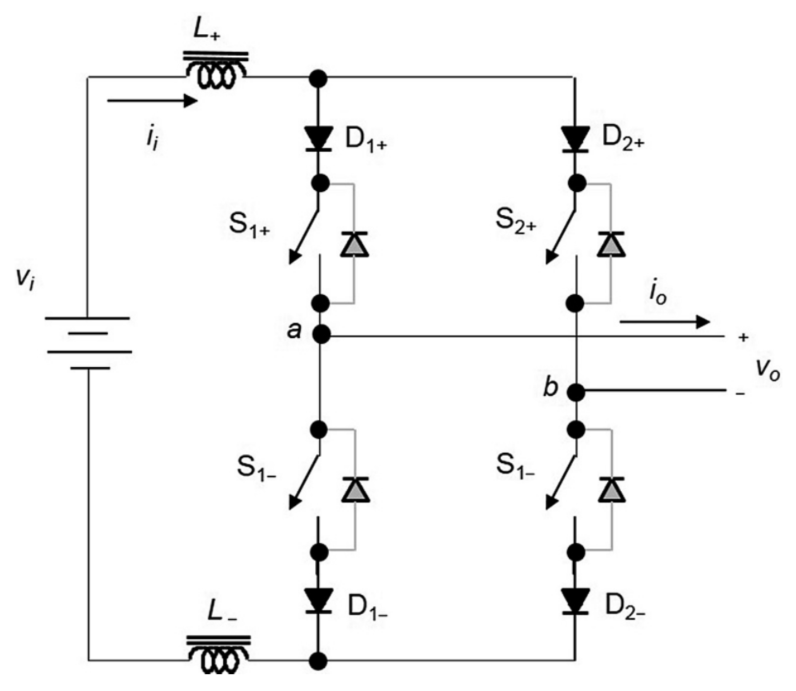
\includegraphics[width=0.6\textwidth]{EMPC_PNG_Pics/CurrentSourceInverter.png}
        \caption{Topology of a singly phase current source inverter, where $V_i$, and $V_o$ are the input and output voltages, $i_i$, and $i_o$ are the input and output currents respectively. $L_+$ and $L_-$ are current filter inductances, $S_{1+}$, $S_{2+}$, $D_{1+}$, and $D_{2+}$ are the higher switches (controlled IGBTs for instance) and diodes, and $S_{1-}$, $S_{2-}$, $D_{1-}$, and $D_{2-}$ are the lower switches and diodes respectively.}
        \label{BASICCSR:fig:SingleCSI}
    \end{figure}

The inductors required are large, such that the inductors
maintain a constant current $i_i$. Current-source topologies feature a low switching $\frac{dV}{dt}$ and reliable over-current or short-circuit protection. In order to operate properly the current-source inverter, we need to adhere to the following rules:
\begin{itemize}
\item Top or bottom switches of the different legs cannot be off simultaneously, because no current path is provided to the input inductors.
\item Diode in series to each switch must be placed, because a short circuit across the output voltage $V_o$ would be produced. If the commercial switch does not include anti- parallel diodes, then the circuit is already complete.
\item In practical implementation, an overlapping time must be considered in the control signals of the top or bottom switches of the different legs.
\end{itemize}

According to the previous rules, it should be noticed that both switches of the inverter leg can be turned on at the same time, and this is not possible in voltage source inverters. There are four ($1^{st}$ to $4^{th}$) defined states of the switches and one not permitted switching state ($5^{th}$ state) as shown in Table \ref{BASICCSR:table:CSIstates}. The modulating technique should always ensure that at any instant, at least one of the top and bottom switch of the inverter legs is on, otherwise the inverter will be damaged.

% Please add the following required packages to your document preamble:
% \usepackage{multirow}
\begin{table}[h!]
\centering
\caption{Switching states of the current source inverter, where $V_{an}$, $V_{bn}$ are the $a$ and $b$ point's potential to ground.}
\begin{tabu}{|c|c|c|c|c|c|c|c|}
\hline
\multicolumn{4}{|c|}{Components conducting} & \multirow{2}{*}{State} & \multicolumn{3}{c|}{Output voltages}                \\ \cline{1-4} \cline{6-8}
$S_{1+}$       & $S_{2+}$       & $S_{1-}$      & $S_{2-}$      &                        & $V_{an}$              & $V_{bn}$              & $V_{o}$           \\ \tabucline[2pt]{-}
1         & 0         & 0        & 1        & 1                      & $V_{i}/2$            & -$V_{i}/2$           & $V_{i}$           \\ \hline
0         & 1         & 1        & 0        & 2                      & -$V_{i}/2$          & $V_{i}/2$            & -$V_{i}$          \\ \hline
1         & 1         & 0        & 0        & 3                      & $V_{i}/2$             & $V_{i}/2$            & 0             \\ \hline
0         & 0         & 1        & 1        & 4                      & -$V_{i}/2$           & -$V_{i}/2$          & 0             \\ \hline
0         & -         & 0        & -        & \multirow{2}{*}{5}     & \multicolumn{3}{c|}{\multirow{2}{*}{Not permitted}} \\ \cline{1-4}
-         & 0         & -        & 0        &                        & \multicolumn{3}{c|}{}                               \\ \hline
\end{tabu}

\label{BASICCSR:table:CSIstates}
\end{table}

The ideal waveforms are shown in Fig.\ref{BASICCSR:fig:CSIwave_A},\ref{BASICCSR:fig:CSIwave_B},\ref{BASICCSR:fig:CSIwave_C}.

\begin{figure}[h!]
                \centering
                \begin{subfigure}[b]{0.9\textwidth}
                    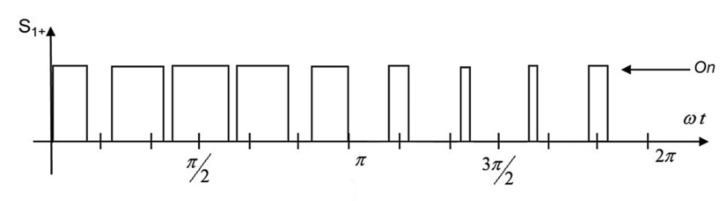
\includegraphics[width=\textwidth]{EMPC_PNG_Pics/CSIwaves_A.png}
                    \caption{\centering The state of switch $S_{1+}$.}
                    \label{BASICCSR:fig:CSIwave_A}
                \end{subfigure}
                ~ %add desired spacing between images, e. g. ~, \quad, \qquad, \hfill etc.
                  %(or a blank line to force the subfigure onto a new line)
                \begin{subfigure}[b]{0.9\textwidth}
                    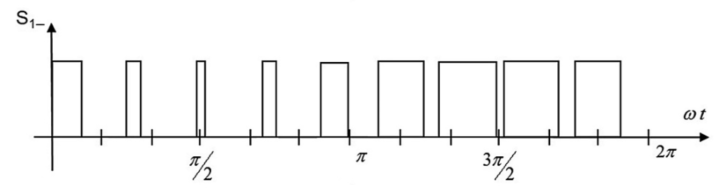
\includegraphics[width=\textwidth]{EMPC_PNG_Pics/CSIwaves_B.png}
                    \caption{\centering The state of switch $S_{2+}$..}
                    \label{BASICCSR:fig:CSIwave_B}
                \end{subfigure}
								 ~ %add desired spacing between images, e. g. ~, \quad, \qquad, \hfill etc.
                  %(or a blank line to force the subfigure onto a new line)
                \begin{subfigure}[b]{0.9\textwidth}
                    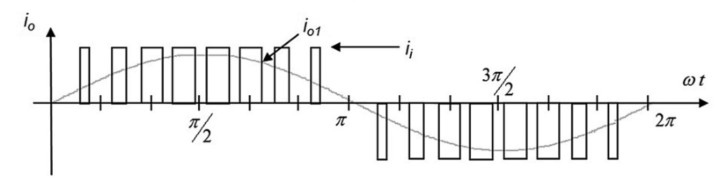
\includegraphics[width=\textwidth]{EMPC_PNG_Pics/CSIwaves_C.png}
                    \caption{\centering AC output current.}
                    \label{BASICCSR:fig:CSIwave_C}
                \end{subfigure}

                \caption{The CSI, ideal waveforms as the result of the modulation.}
            \end{figure}

The states for the switches are defined by the modulating technique, which in this case is a carrier-based PWM, but unipolar output is considered. For the CSIs, different output filters may be employed, in order to provide the fundamental component of the output waveform. Depending on the application, it would be desirable to provide a voltage or current output.

\subsection{Galvanic decoupled bi-directional DC-DC converters}\label{BASICCSR:sec:DCDC}

In this section a basic galvanic decoupled voltage source DC-DC converter shall be presented. In many DC power supplies, a galvanic isolation between the DC or AC input and the DC output is required for safety and reliability. An economical mean of achieving such an isolation is to employ a transformer version of a DC-DC converter. High-frequency transformers are of a small size and weight and provide high efficiency. Their turns ratio can be used to additionally adjust the output voltage level. Generally, electric power generated by renewable energy sources is unstable in nature, thus producing a bad effect on the utility grid. This fact motivates research on energy storage and quality systems to smooth out active-power flow.\\
On Fig.\ref{BASICCSR:fig:DCDCGalvanic} the converter has two symmetrical single-phase voltage-source full-bridge converters, allowing a bi-directional power flow. Thanks to advancement in power device technology over the last decade has enabled the DC-DC devices to operate at an efficiency as high as $\approx97\%$ by using the latest trench-gate IGBTs. Therefore this topology has become a promising candidate as a power electronic interface for an energy storage and renewable system \cite{kheraluwala1992performance} \cite{inoue2007bidirectional}.


\begin{figure}[!ht]
        \centering
        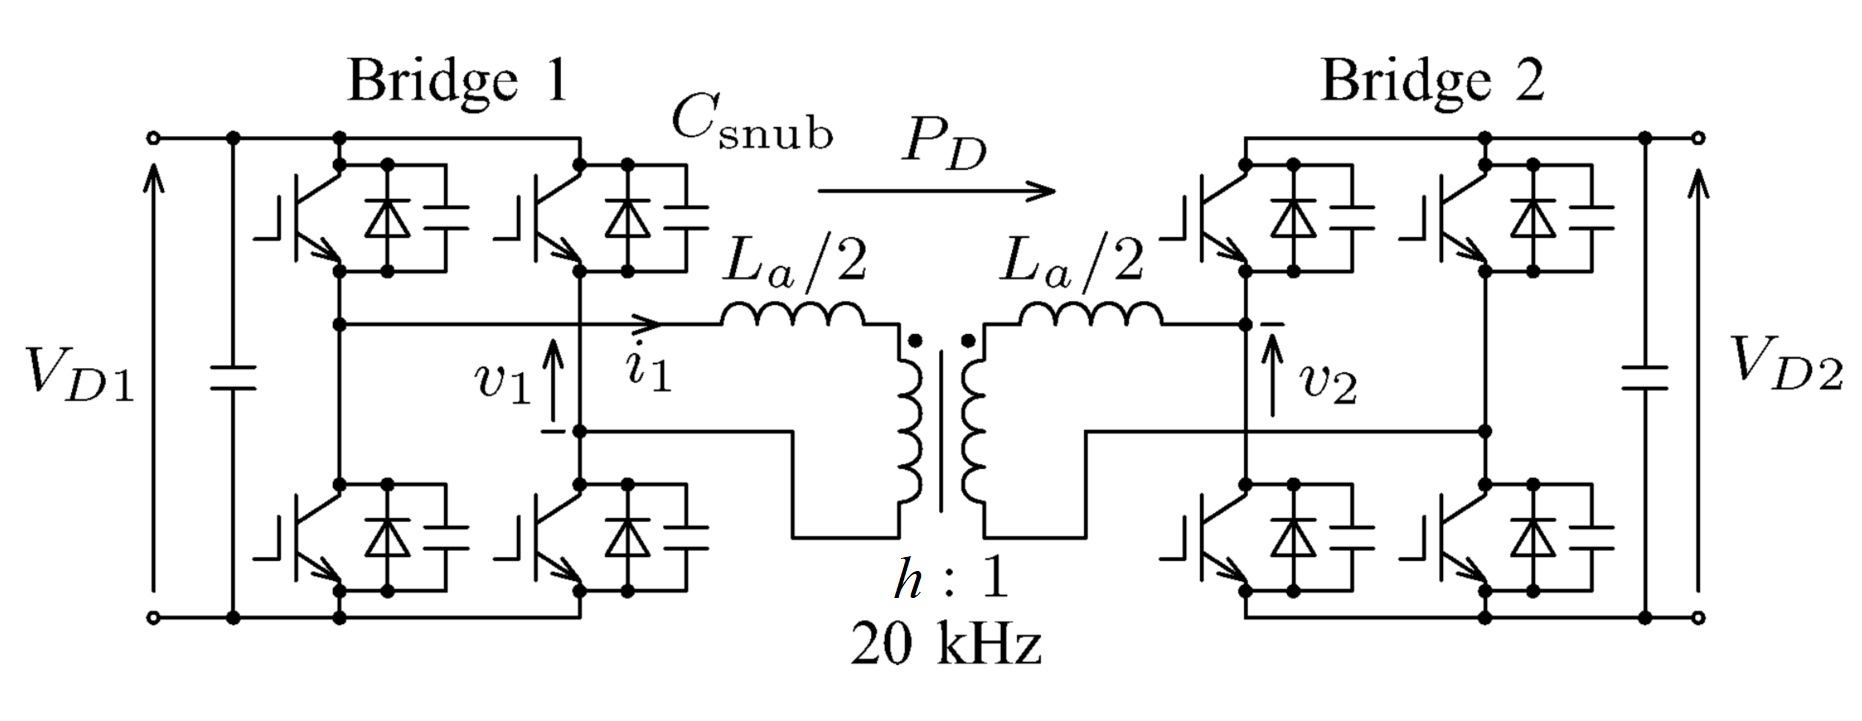
\includegraphics[width=0.7\textwidth]{EMPC_PNG_Pics/DC_DC_galvanic.png}
        \caption{Bidirectional isolated DC-DC converter, where $V_{D1}$, and $V_{D2}$ are the two end's voltage (in- and output depends on the power flow), $v_1$ and $v_2$ are the transformer voltages, $C_{snub}$ are to reduce switching loss and to damp out
over-voltage, and $n$ is the transformer turn ratio.}
        \label{BASICCSR:fig:DCDCGalvanic}
    \end{figure}
		
The principle of operation of the DC-DC converter is very simple. Two active bridges are interfaced through a transformer and are phase shifted from each other to control the amount of power flow from one DC voltage source to the other. This allows a fixed frequency, square-wave mode of operation and utilization of the leakage inductance of the transformer as the main energy transfer element. The power transfer under idealized conditions is defined as:

\begin{equation}
        \begin{array}{rcl}
            P_D&=&\frac{V_{D1}V_{D2}}{\omega L}\left(\delta-\frac{\delta^2}{\pi}\right)\\
        \end{array}
        \label{BASICMPC:equ:DCDC}
    \end{equation}
		
		where $\omega=2\pi f$ is the switching angular frequency of the two single phase full bridge controllers, $L_a$ is the
sum of the transformer leakage inductance.

\subsection{Three-phase buck-type rectifiers}\label{BASICCSR:sec:CSR}

Three-phase controlled rectifiers have a wide range of applications, from small rectifiers to large high-voltage direct-current
transmission systems. They are used for electrochemical processes, many kinds of motor drives, traction equipment, controlled power supplies, and many other applications. In this thesis only force commuted rectifiers are examined, which are built with semiconductors (IGBTs in this case) with gate-turn-off capability. The gate-turn-off capability allows full control of the converter, because valves can be switched ON and OFF whenever is required. This allows the commutation of the valves, hundreds of times in one period that is not possible with line-commutated rectifiers, where IGBTs are switched ON and OFF only once a cycle. This has the following advantages:

\begin{itemize}
\item The current or voltage can be (pulse width) modulated, generating less harmonic contamination.
\item The power factor can be controlled and even it can be made leading.
\item They can be built as voltage-source or current-source based on the required application.
\item The reversal of power in switching rectifiers is by reversal of voltage at the DC link. This allows force commutated rectifiers can be implemented for both, reversal of voltage or reversal of current.
\end{itemize}

There are two ways to implement force commutated three phase rectifiers, as a current-source rectifier (Fig.\ref{BASICMPC:fig:CSR}), where power reversal is by DC voltage reversal, and as a voltage-source rectifier (Fig.\ref{BASICMPC:fig:VSR}), where power reversal is by current reversal at the DC link.


\begin{figure}[h]
                \centering
                \begin{subfigure}[b]{0.9\textwidth}
                    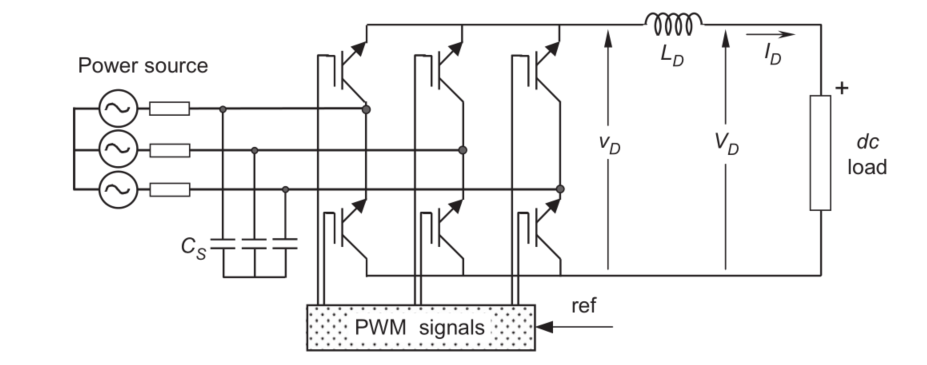
\includegraphics[width=\textwidth]{EMPC_PNG_Pics/BasicCurrentRectifiers.png}
                    \caption{\centering Current source rectifier with capacitive filtering and choke inductance.}
                    \label{BASICMPC:fig:CSR}
                \end{subfigure}
                ~ %add desired spacing between images, e. g. ~, \quad, \qquad, \hfill etc.
                  %(or a blank line to force the subfigure onto a new line)
                \begin{subfigure}[b]{0.9\textwidth}
                    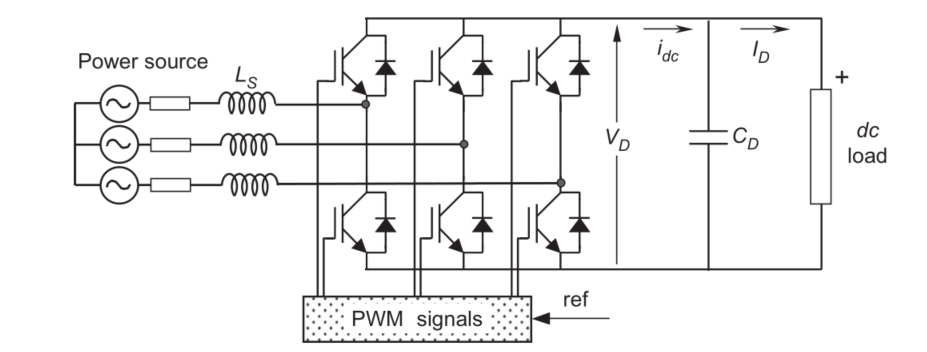
\includegraphics[width=\textwidth]{EMPC_PNG_Pics/BasicVoltageRectifiers.png}
                    \caption{\centering Voltage source rectifier with inductive filtering and DC voltage smoothing capacitance.}
                    \label{BASICMPC:fig:VSR}
                \end{subfigure}
                 %add desired spacing between images, e. g. ~, \quad, \qquad, \hfill etc.
                %(or a blank line to force the subfigure onto a new line)
                %\begin{subfigure}[b]{0.48\textwidth}
                    %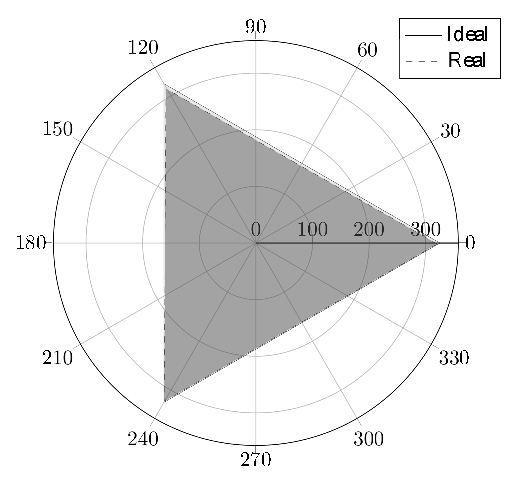
\includegraphics[width=\textwidth]{Unblance_EPS_Pics/EPS_images/square.eps}
                    %\caption{Low correlation with opposed amplitude deviation. The norm values are $G=9322$ and $TDV=0.5198$.}
                    %\label{fig:cases_C}
                %\end{subfigure}
                %~
                %\begin{subfigure}[b]{0.48\textwidth}
                    %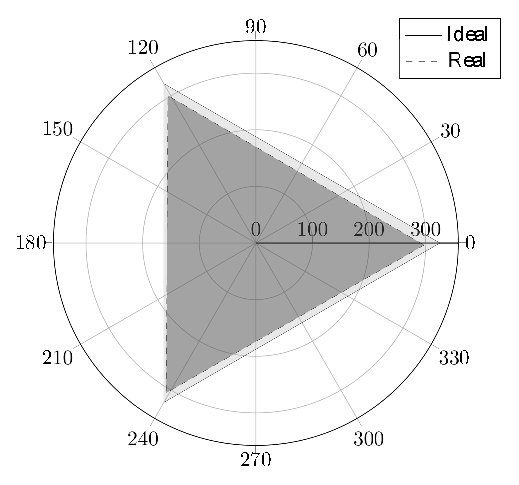
\includegraphics[width=\textwidth]{Unblance_EPS_Pics/EPS_images/circle.eps}
                    %\caption{\centering Low correlation with uniform voltage drop. The norm values are $G=6280$ and $TDV=0.156$.}
                    %\label{fig:cases_D}
                %\end{subfigure}


                \caption{Basic topologies of force commuted rectifiers.}
            \end{figure}

%\begin{figure}[!ht]
        %\centering
        %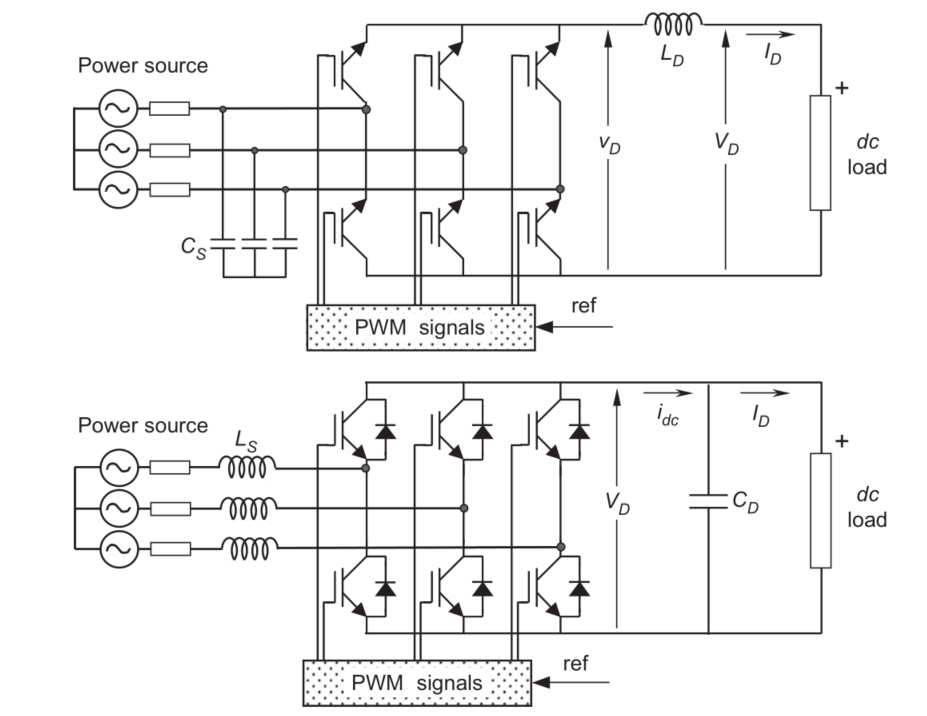
\includegraphics[width=0.9\textwidth]{EMPC_PNG_Pics/CurrentVoltageRectifiers.png}
        %\caption{Basic topologies of force commuted rectifiers.}
        %\label{BASICCSR:fig:topologies}
    %\end{figure}


As  general case a front-end  converter power supply (e.g. lighting or telecommunications) shall designed that should have approximately these general characteristics: sinusoidal main currents, unity power factor, high power density and simplicity of the power circuit structure. Two structures are most fitted for the task. First a boost-type input rectifier (e.g., Vienna rectifier, \cite{kolar1996design}), that typically features two $400V$ output voltages with a three-level isolated  DC-DC  converter  or  two  isolated  DC-DC  output  stage (see Fig. \ref{EMPC:fig:network} in Ch.5.). The second candidate is the buck-type  input  rectifier (or current source rectifier (CSR))  (conventionally  six-switch topologies as proposed in \cite{zargari1993current}, \cite{sato1993state}) with only one two-level isolated  DC-DC  converter  output  stage.  Also the  input  stage  can be realized as a three-switch topology with considerably  lower  system  complexity  as  compared  to  the boost-type structure. In particular, the number of utilized active and passive components is much lower. Furthermore, there is no middle-point that has to be stabilized, as this is the case for the boost-type structures, making control and active filter design less complex. Further system advantages are the potential of direct start-up and the implicit over current protection in case of an output short circuit. Therefore, this topologies of high interest for many safety critical applications as such future electric aircraft, or automotive applications or as power supplies for process technology \cite{nussbaumer2007comprehensive}.
The three-switch buck rectifier topology was first proposed in \cite{malesani1987three}. In \cite{itoh1989steady} and \cite{tooth2000effects}, aspects of the system modulation and control have been treated. The application of the topology used as an active filter is discussed in \cite{salo2005three}.  The addition of a DC-DC output boost-stage has been proposed in \cite{baumannnew} in order to maintain 400 V output voltage for a wide input voltage range and for the case of unbalanced mains as, e.g., the loss of one phase.

\myparagraph{Basic operation principles}\label{BASICCSR:sec:OperationPrinciple}

For the derivation of the relative on-times of the three buck transistors $S_i$ with the following assumptions are made for clarity and facilitation of calculations:
\begin{itemize}
	\item The AC-side filter capacitor voltages ($v_{c_p}$, where $p\in\{1,2,3\}$) at the input of the CSR are sinusoidal and in phase with the main harmonic component of voltage.
	
	\begin{equation}
        \begin{array}{rcl}
            v_{c_1}&=&\widehat{v}_ccos(\omega t)\\
						v_{c_2}&=&\widehat{v}_ccos(\omega t-2\pi/3)\\
						v_{c_3}&=&\widehat{v}_ccos(\omega t+2\pi/3),\\
        \end{array}
        \label{BASICMPC:equ:phasorvect}
    \end{equation}
	where $\omega$ is the network voltage's angular velocity.
	
	\item The mains currents are assumed to be equal to the fundamental component of the rectifier input currents.
	\item The current in the DC output inductor $L_{D}$ is not affected by the high frequency ripple due to the switching operation.
\end{itemize}

 For achieving ohmic mains behavior also in case of unbalanced fundamental harmonics conditions the explained modulation method can still be utilized, however, additionally the control structure presented in \cite{baumann2005novel} has to be employed.\\
The waveforms of the phase and line-to-line mains voltages are divided into twelve $30°$ wide sectors shown in Fig.\ref{BASICCSR:fig:waves}. The following calculations are based on the analysis of the first sector which is characterized by the voltage harmonic phase relation. For the remaining sectors the calculations can be accomplished in an similar manner \cite{nussbaumer2007comprehensive}.

\begin{figure}[!ht]
        \centering
        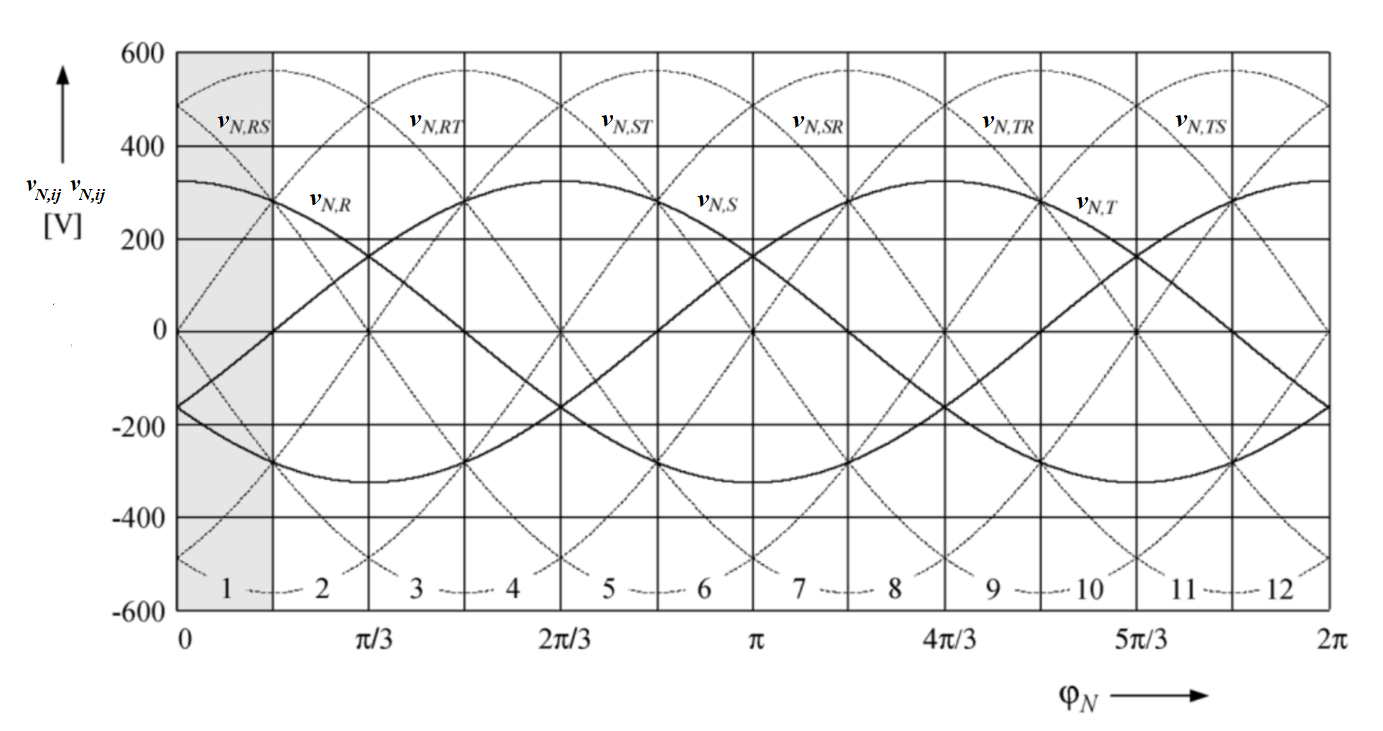
\includegraphics[width=\textwidth]{EMPC_PNG_Pics/Waves.png}
        \caption{Phase voltages $v_{i}$, where line-to-line voltages $v_{N,ij}=v_{N,i}-v_{N,j}$, $(i,j)\in\{R,S,T\}$ and sectors $1$ to $12$ being defined by the different relations of the instantaneous values of the mains phase voltages for $v = 400 V$}
        \label{BASICCSR:fig:waves}
    \end{figure}
		
		Accordingly, on AC side, if conditions are favorable, inductor current can appear in an instant of time either in two out
of three phases or in none. In this modulation technique, the switches in each converter leg can conduct only one at the time (aside from zero states, where both upper and lower switches are conducting). When the upper leg is conducting it is indicated by `$1$', when the lower  `$-1$' and when neither `$0$'. As such the choice whether upper or lower switch of the leg conducts current depends of the reference current vector's sector location.
According to the actual switch combination the DC link current shaped by the choke inductance, and distributed to two of the input phases or the freewheeling diode. With this, the input current space vectors can be calculated for each of the before-mentioned switching states. Generally the space vector of three-phase quantities (e.g., for the rectifier input current) are described as:

\begin{equation}
        \begin{array}{rcl}
            \vec{i}&=&\frac{2}{3}\left(\vec{i}_a+\vec{i}_be^{\frac{j\pi}{3}}+\vec{i}_bc^{\frac{4j\pi}{3}}\right).\\
        \end{array}
        \label{BASICCSR:eqn:currents}
    \end{equation}
		
		Based on \ref{BASICCSR:eqn:currents} the corresponding active space vectors in the first sector can be obtained as:
		
		\begin{equation}
        \begin{array}{rcl}
            \vec{i}_{(1,0,-1)}=\vec{i}_1&=&2i_{dc}e^{j\pi/6}/\sqrt{3}\\
						\vec{i}_{(0,1,-1)}=\vec{i}_2&=&2i_{dc}e^{j\pi/2}/\sqrt{3}\\
						\vec{i}_{(-1,1,0)}=\vec{i}_3&=&2i_{dc}e^{j5\pi/6}/\sqrt{3}\\
        \end{array}
        \label{BASICCSR:eqn:currents}
    \end{equation}
		
		The resulting discrete space vectors can be used to synthesize desired current
space vector $\vec{i}_{ref}$.

The modulation methods were evaluated in and chosen for this paper based on \cite{moussaoui2005open}, which ensures minimum switching-losses, minimum ripple values of the input capacitor voltages and of the output inductor current. According to this modulation, each pulse interval comprises two active states and a freewheeling state, arranged symmetrically about the middle of the pulse interval (see Table \ref{EMPC:tbl:sequence}). For more in depth functional description see section \cite{EMPC:sec:Modulation}.

\section{Applied optimization methods}

In this part of the thesis, the applied control structures shall be discussed in detail. Optimization (or optimal control) deals with the problem of finding a control law for a given system such that a certain optimality criterion is achieved. A control problem includes a cost functional that is a function of state and control variables. An optimal control is a set of differential equations describing the paths of the control variables that minimize the cost function. They commonality in this work, is that all of them are designed to search for the optimal control input for a current governing system, should it be voltage unbalance reduction with no applicable network model (due the actors unpredictability), or reaching the fastest reference value with explicit predictive control with the converter's equation's considered.

\subsection{Asynchronous parallel pattern search}\label{BASICUNB:sec:APPS}

This algorithm can rather be described as a linear search program, distributed in a multi-dimensional plane, where the it is only a black box model available. These variants of pattern search can solve nonlinear unconstrained problems of the form of:

\begin{equation}
        \begin{array}{rcl}
            \min_{x\in\mathbb{R}^n}f(x),\\
        \end{array}
        \label{BASICCSR:eqn:currents}
    \end{equation}
		
		where $f:\mathbb{R}^n\longrightarrow\mathbb{R}$. We assume that the evaluation of $f$ is computationally expensive, hence our interest in using either distributed or parallel computing environments to solve the problem. It needs to be concentrated on the parallelization of the search strategy, rather than on the evaluation of $f$, though the techniques we discuss here can be adapted to handle problems for which the computation of $f$ also can be distributed. Additionally is is assumed that $f$ is continuously differentiable, we further assume that $\nabla f$ is unavailable
and not reliable. For such problems, pattern search methods are one possible solution technique since they neither require nor explicitly estimate derivatives.\\

\myparagraph{Parallel pattern search}

Lets adopt an infinite sequence of iterations $\rho=0,1,2,\dots$, with the last iteration noted as $\rho-1$ and initialization at $0$. It is assumed that the process knows the best point so far as $x^{\rho-1}$, where $f(x^{\rho-1})$ has the global minima of $f$. Associated with $x^{\rho-1}$ there is a step-length control parameter namely $\Delta^{\rho-1}$. Each $i\in\mathcal{P}$, where $\mathcal{P}=\{1,\dots,p\}$ process ends iteration at $\rho-1$ by constructing it's trial point and initiating an evaluation of $f(x^{\rho-1}_i+\Delta^{\rho-1}_id_i)$, where $\mathcal{D}=\{d_1,\dots,d_p\}$ is the finite set of directions applied by each individual process. The simultaneous start of the function evaluations at the trial points on each of the $p$ processes signals the start of iteration $\rho$. When all of the participating processes are finished with their evaluation of $f$, they communicate these values to each other and determine the new values of $x^\rho$, and $\Delta^\rho$. If there exists an $i\in\mathcal{P}$, such that $f(x^{\rho-1}_i+\Delta^{\rho-1}_id_i)<f(\rho^{\rho-1})$, then $\rho\in\mathcal{S}$, where $\mathcal{S}$ denotes the successful iterations.

\myparagraph{Adding asynchronicity}

 With said above, the general strategy for asynchronous parallel pattern search, from the perspective of a single process $i\in\mathcal{P}$ can be outlined:
		\begin{enumerate}
		\item Evaluate $f(x^{best}_i+\Delta^{best}_id_i)$.
		\item If $f(x^{best}_i+\Delta^{best}_id_i) <f(x^{best}_i)$, then broadcast result to all other processes.
		\item Update local values $x^{best}_i$ and $\Delta^{best}_i$ based on the current local information.
		\item Repeat.
		\end{enumerate}
	The price payed is that each process has its own notion of the best known point seen so far, as well as its own value for	$\Delta^i$. Any success on one process is communicated to all other processes participating in the search, but the successful process carries on from its new best point without waiting for a response from the other processes. By adding a few mild conditions, the global convergence of the search can be still ensured \cite{kolda2003understanding}.  Instead of indexing based on a notion of iterations, we switch from $\rho$ to indexing based on discrete time instance, letting the set $\mathcal{Q}=\{1,2,\dots,q\}$ denote the index if steps. Thus $x_i^q$ s used for the best point known to process $i$ at time step $q$, and similarly, $\Delta_i^q$.  So if process $i$ starts a function evaluation at time step $q$, the trial point at which the function evaluation will be made at $x^{q}_i+\Delta^{q}_id_i$. Further worth mention, that time steps are assumed to be of fine enough resolution so that at most one function evaluation finishes per process per time step.\\
	Lets define two sets that satisfy $\mathcal{Q}=\mathcal{S}_i\cup\mathcal{U}_i$, , and $\mathcal{S}_i=\mathcal{I}_i\cup\mathcal{E}_i$, where $\mathcal{S}_i$ is the set of all time successful steps on process $i$, $\mathcal{I}_i$ is the set if internal successes, $\mathcal{E}_i$ is the set of external successes,   and $\mathcal{U}_i$ consists the unsuccessful steps respectfully. An internal success, where the process finds itself the minima, the external sucess is where the process is updated externally by the minima. Further  $\mathcal{C}_i\in\mathcal{U}_i$ is defined as the set of time steps where $\Delta^t_i$ is reduced. All the above cases ($\mathcal{U}_i\textbackslash\mathcal{C}_i$) no action is performed.\\
	The updating functions allow us to give the following general definitions for $x_i^q$ and $\Delta^q_i$. For every $q\in\mathcal{Q}$, $q>0$, the best pont for the $i^{th}$ process defined to be:
	
	\begin{equation}
        \begin{array}{rcl}
            x_i^q&=&\begin{Bmatrix}
                x_{\omega_i(q)}^{\tau_i(q)}+\Delta_{\omega_i(q)}^{\tau_i(q)}d_{\omega_i(q)},&\textnormal{if }q\in\mathcal{S}_i\\
                x_i^{q-1},&\textnormal{otherwise}\\
            \end{Bmatrix},\\
        \end{array}
        \label{BSIC:equ:APPS_x}
    \end{equation}
		
		with the initialisation $x^0_i=x^0$, where $\omega_i(q)$ is the generating process index for the update time at step $q$ on process $i$, and $\tau_i(q)$ is the time index for initialization of the function evaluation, that produced the update at time $q$ on process $i$. For every $q$ the step lenght control parameter $\Delta_i^q$ defined to be:
		
		\begin{equation}
        \begin{array}{rcl}
            \Delta_i^q&=&\begin{Bmatrix}
                \lambda_{\omega_i(q)}^{\nu_i(q)}\Delta_{\omega_i(q)}^{\tau_i(q)},&\textnormal{if }q\in\mathcal{S}_i\\
								\theta_{i}^{q}\Delta_{\omega_i(q)}^{\tau_i(q)},&\textnormal{if }q\in\mathcal{C}_i\\
                \Delta_i^{q-1},&\textnormal{otherwise}\\
            \end{Bmatrix},\\
        \end{array}
        \label{BSIC:equ:APPS_Delta}
    \end{equation}
		
		with the initialization $\Delta^0_i=\Delta^0$, where $\nu_i(q)$ is  time index for the completion of the function evaluation that produced the update at time step $q$ on process $i$, and $\theta_i^q$ and $\lambda_i^q$ are choosen. With the following pattern followed, the minima of $f$ shall eventually reached, in an undetermined steps \cite{kolda2003understanding}.

\subsection{Quadratic optimization and predictive control}\label{BASICCSR:sec:MPC}

Philosophically MPC reflects human behavior whereby we select control actions which we think will lead to the best predicted outcome (or output) over some limited horizon. To make this selection we use an internal model of the process in question, and constantly update our decisions as new observations become available. Hence a predictive control law has the following components:
\begin{itemize}
\item The control law depends on predicted behavior.
\item The output predictions are computed using a process model.
\item The current input is determined by optimizing some measure of predicted performance.
\item The receding horizon: the control input is updated at every sampling instant.
\end{itemize}

%\myparagraph{Model predictive control}\label{BASICCSR:sec:MPCOverview}
Most control laws, say PID (proportional, integral and derivative) control, does not explicitly consider the future implication of current control actions. To some extent this is only accounted by the expected closed-loop dynamics. MPC on the other hand
implicitly (or explicitly) computes the predicted behavior over some horizon. One can therefore restrict the choice of the proposed input trajectories to those that do not lead to difficulties in the future.\\
In order to predict the future behavior of a process, we must have a model of how the process behaves. In particular, this model must show the dependence of the output on the current measured variable and the current/future inputs. This does not have to be linear (e.g. transfer function, state-space) and in fact can be just about anything. A precise model is not always required to get tight control, because the decisions are updated regularly. This will deal with some model uncertainty in a fairly fast time scale. The decision on the best control is thus continually updated using information from this comparison \cite{rossiter2017model}.\\
This way, model based predictive control methods are optimal regulators, with a defined cost function on a defined and encompassed prediction horizon with restrictions \cite{kwon2006receding}, \cite{baotic2005optimal}, \cite{herceg2009real}, \cite{grancharova2005survey}. The control signal is calculated over a defined horizon, but from the sequence of applicable control signals only the first one is used in the next sample. This procedure is repeated according to the principle of the moving horizon, using new iterations, as such provides the reaction in each sample. The method was developed for systems with physical restrictions, in the first stage for the control of chemical processes in the oil industry, then it was applied to various rapid processes from automotive or power electronics industry \cite{antoniewicz2009predictive} , \cite{geyer2005low}. By default the optimization problem can be solved, for each sample, or explicitly using the multi-parameter programming techniques (mp-LP, mp-QP).% presented in \textbf{[N-ANNEX 1]-(Needed?)}, over a well-defined parameter space.

	\myparagraph{Linear quadratic optimal control}\label{BASICCSR:sec:LQR}

In practice most MPC algorithms use linear models because the dependence of the predictions on future control choices is then linear and this facilitates optimization as well as off-line analysis of expected closed-loop behavior. However, nonlinear models can be used where the implied computational burden is not a problem and linear approximations are not accurate enough. It is also important to note here the comment fit for purpose. In predictive control, the model is used solely to compute system output predictions, so the model is fit for purpose if it gives accurate enough predictions. The effort and detail put into modeling stage should reflect this.	Let the us assume that the system is linear and time-invariant (LTI):
	
	    \begin{equation}
        \begin{array}{rcl}
            \textbf{x}(q+1)&=&\textbf{Ax}(q)+\textbf{Bu}(q),\\
						%\textbf{y}(q)&=&\textbf{Cx}(q)
        \end{array}
        \label{BASICMPC:equ:basic_LTI}
    \end{equation}

    where $\textbf{x}(q)\in\mathbb{R}^n$ and $\textbf{u}(q)\in\mathbb{R}^m$ are the state and input vectors respectively. We define a quadratic coat function over a finite horizon of $N$ steps:

  %  \begin{equation}
%        \begin{array}{rcl}
%				%&&\norm{asd}
%         J_0(\textbf{U}_n,\textbf{x}(0))&=&\norm{{\textbf{Px}_N}}_\varsigma+\sum^{N-1}_{k=0}\norm{\textbf{Qx}_k}_\varsigma+\norm{\textbf{Ru}_k}_\varsigma\\
%        \end{array}
%        \label{BASICMPC:equ:cost_function}
%    \end{equation}

    %Let's assume system \ref{BASICMPC:equ:basic_LTI} with applied cost function \ref{BASICMPC:equ:cost_function}, and optimization problem \ref{BASICMPC:equ:optim_problem}. If we assume Euclidian norm ($\varsigma = 2$) the cost function can be written in the following way:


\begin{equation}
        \begin{array}{rcl}
				%&&\norm{asd}
         J_0(\textbf{U}_0,x(0))&=&\textbf{x}'_N\textbf{P}\textbf{x}_N+\sum^{N-1}_{k=0}\textbf{x}'_k\textbf{Q}\textbf{x}_k+\textbf{u}'_k\textbf{R}\textbf{u}_k\\
        \end{array}
        \label{BASICMPC:equ:cost_function_Euclidian}
    \end{equation}

    where $U_0=[\textbf{u}'_0,\dots,\textbf{u}'_{N-1}]in\mathbb{R}^s$, $s=m*N$ is the decision vector constraining all future inputs, also $\textbf{P}=\textbf{P}'\succeq 0$, $\textbf{Q}=\textbf{Q}'\succeq 0$, $\textbf{R}=\textbf{R}'\succeq 0$, and $\textbf{x}_k$ denotes the state vector at time $k$ obtained form $\textbf{x}_0=\textbf{x}(0)$. We also apply the system model based on \ref{BASICMPC:equ:basic_LTI}:

    \begin{equation}
        \begin{array}{rcl}
            \textbf{x}_{k+1}&=&\textbf{Ax}_k+\textbf{Bu}_k,\\
						%\textbf{y}(q)&=&\textbf{Cx}(q)
        \end{array}
        \label{BASICMPC:equ:basic_horizon model}
    \end{equation}

   From the above a finite optimal control problem can be considered:

   \begin{equation}
        \begin{array}{rcl}
				%&&\norm{asd}
         J^*_0(\textbf{x}(0))&=&\min_{\textbf{U}_0}J_0(\textbf{U}_0,x(0))\\
         &\textnormal{subj. to}&\textbf{x}_{k+1}=\textbf{Ax}_k+\textbf{Bu}_k\\
         &&\textbf{x}_0=\textbf{x}(0)\\
         &&k=0,1,\dots,N-1
        \end{array}
        \label{BASICMPC:equ:optimal_control_problem_Euclidian}
    \end{equation}


    The first step is to write the equality constraints to express all future states and inputs from the initial state $\textbf{x}_0$ until the and of horizon $N$:

    \begin{equation}
        \begin{array}{rcl}
        \underbrace{
        \begin{bmatrix}
        \textbf{x}(0)\\
        \textbf{x}_1\\
        \vdots\\
        \vdots\\
        \textbf{x}_N\\
        \end{bmatrix}}_{\mathcal{X}^x}
        &=&
        \underbrace{
        \begin{bmatrix}
        \textbf{I}_0\\
        \textbf{A}_1\\
        \vdots\\
        \vdots\\
        \textbf{A}^N\\
        \end{bmatrix}}_{\mathcal{S}^x}\textbf{x}(0)+
        \underbrace{
        \begin{bmatrix}
        0& \dots& \dots& 0\\
        \textbf{B}& 0& \dots& 0\\
        \textbf{AB}& \ddots& \ddots& \vdots\\
        \vdots& \ddots& \ddots& \vdots\\
        \textbf{A}^{N-1}\textbf{B}& \ddots& \ddots& \textbf{B}\\
        \end{bmatrix}}_{\mathcal{S}^u}
        \begin{bmatrix}
        \textbf{u}_0\\
        \vdots\\
        \vdots\\
        \textbf{u}_N\\
        \end{bmatrix}.

		\end{array}
        \label{BASICMPC:equ:batch_allstates}
    \end{equation}

    %For the easier notation it is asmued that $\mathcal{X^x}={\textbf{x}(0),\textbf{x}_1,\dots,\textbf{x}_N}$, $\mathcal{S^x}={\textbf{I},\textbf{A},\dots,\textbf{x}_N}$ $ \underbrace{(x + 2)^3}_{\text{text 1}}$
    Here all future states are explicit functions of the state $\textbf{x}(0)$ and the future inputs of $\textbf{u}_0,\textbf{u}_1\cdot$ only. By defining appropriate quantities, we can rewrite \ref{BASICMPC:equ:batch_allstates} in a compact form:

    \begin{equation}
        \begin{array}{rcl}
        \mathcal{X}^x&=&\mathcal{S}^x(0)+\mathcal{S}^u\textbf{U}_0.\\
		\end{array}
        \label{BASICMPC:equ:batch_allstates_compact}
    \end{equation}

    Using the same notation the object function can be rewritten as:

    \begin{equation}
        \begin{array}{rcl}
        J(\textbf{x}_0,\textbf{U}_0)&=&\mathcal{X}'\bar{\textbf{Q}}\mathcal{X}+\textbf{U}_0\bar{\textbf{Q}}\textbf{U}'_0,\\
		\end{array}
        \label{BASICMPC:equ:batch_object}
    \end{equation}

    where $\bar{\textbf{Q}}=diag\{\textbf{Q},\dots,\textbf{Q},\textbf{P}\}$, and $\bar{\textbf{R}}=diag\{\textbf{R},\dots,\textbf{R}\}$. Substituting \ref{BASICMPC:equ:batch_allstates_compact} into the objective function \ref{BASICMPC:equ:batch_object} yields:

    \begin{equation}
        \begin{array}{rcl}
        J(\textbf{x}_0,\textbf{U}_0)&=&(\mathcal{S}^x(0)+\mathcal{S}^u\textbf{U}_0)'\bar{\textbf{Q}}(\mathcal{S}^x(0)+\mathcal{S}^u\textbf{U}_0)+\textbf{U}_0'\bar{\textbf{R}}\textbf{U}_0\\
        &=&\textbf{U}'_0\underbrace{(\mathcal{S}^{u'}\bar{\textbf{Q}}\mathcal{S}^u+\bar{\textbf{R}})}_{\textbf{H}}\textbf{U}_0+ \\
        &+&2\textbf{x}'(0)\underbrace{(\mathcal{S}^{x'}\bar{\textbf{Q}}\mathcal{S}^u)}_{\textbf{F}}\textbf{U}_0+\\
        &+&\textbf{x}'(0)\underbrace{(\mathcal{S}^{x'}\bar{\textbf{Q}}\mathcal{S}^x)}_{\textbf{Y}}\textbf{x}(0)\\
        &=&\textbf{U}'_0\textbf{H}\textbf{U}_0+2\textbf{x}'(0)\textbf{F}\textbf{U}_0+\textbf{x}'(0)\textbf{Y}\textbf{x}(0).
		\end{array}
        \label{BASICMPC:equ:batch_simplfy}
    \end{equation}

    Because $\bar{\textbf{R}}\succ 0$, and $\bar{\textbf{H}}\succ 0$, thus $J(\textbf{x}_0,\textbf{U}_0)$ is a positive definite quadratic function of $\textbf{U}_0$, therefore its minimum can be found by computing its gradient and setting it to zero, which yields the optimal vector of future inputs:
%
    \begin{equation}
        \begin{array}{rcl}
        \textbf{U}^*_0(\textbf{x}(0))&=&-\textbf{H}^{-1}F'x(0)\\
        &=&-(\mathcal{S}^{u'}\bar{\textbf{Q}}\mathcal{S}^{u}+\bar{\textbf{R}})^{-1}\mathcal{S}^{u'}\bar{\textbf{Q}}\mathcal{S}^{x}\textbf{x}(0).
		\end{array}
        \label{BASICMPC:equ:batch_optimal_solution}
    \end{equation}

    With \ref{BASICMPC:equ:batch_optimal_solution} applied and calculated $\textbf{U}_0$ the cost is the optimal following:

    \begin{equation}
        \begin{array}{rcl}
        \textbf{J}^*_0(\textbf{x}(0))&=&-\textbf{x}(0)'\textbf{F}\textbf{H}^{-1}F'x(0)\\
        &=&\textbf{x}(0)'\left[ \mathcal{S}^{x'}\bar{\textbf{Q}}\mathcal{S}^{x} - \mathcal{S}^{x'}\bar{\textbf{Q}}\mathcal{S}^{u}
        (\mathcal{S}^{u'}\bar{\textbf{Q}}\mathcal{S}^{u}+\bar{\textbf{R}})^{-1}\mathcal{S}^{u'}\bar{\textbf{Q}}\mathcal{S}^{x}  \right]\textbf{x}(0).
		\end{array}
        \label{BASICMPC:equ:batch_optimal_cost}
    \end{equation}

    Note that the optimal vector of future inputs $\textbf{U}^*_0(\textbf{x}(0))$ is a linear function of \ref{BASICMPC:equ:batch_optimal_solution} of the initial state $\textbf{x}(0)$ and the optimal cost $J^*_0(x(0))$ is a quadratic function \ref{BASICMPC:equ:batch_optimal_cost} of the initial state $\textbf{x}(0)$.\\
    Alternatively the formulation can be done in a recursive manner. The optimal cost can be defined as $J^*_j(\textbf{x}_j)$ fot the $j^{th}$ for the $N-j$ step problem starting from state $\textbf{x}_j$ as:

    \begin{equation}
        \begin{array}{rcl}
				%&&\norm{asd}
         J^*_j(\textbf{x}_j)&=&\min_{\textbf{u}_j,\dots,\textbf{u}_{N-1}}\textbf{x}'_N\textbf{P}\textbf{x}_N+\sum^{N-1}_{k=0}\textbf{x}'_k\textbf{Q}\textbf{x}_k+\textbf{u}'_k\textbf{R}\textbf{u}_k.\\
        \end{array}
        \label{BASICMPC:equ:cost_function_Euclidian_recursive}
    \end{equation}

    The optimal "one step cost to go" can be obtained as:

     \begin{equation}
        \begin{array}{rcl}
				%&&\norm{asd}
         J^*_{N-1}(\textbf{x}_{N-1})&=&\min_{\textbf{u}_{N-1}}\textbf{x}'_N\textbf{P}_N\textbf{x}_N+\textbf{x}'_{N-1}\textbf{Q}\textbf{x}_{N-1}+\textbf{u}'_{N-1}\textbf{R}\textbf{u}_{N-1}.\\
          &\textnormal{subj. to}&\textbf{x}_N=\textbf{Ax}_{N-1}+\textbf{Bu}_{N-1}\\
          &&\textbf{P}_N=\textbf{P},\\
        \end{array}
        \label{BASICMPC:equ:cost_function_Euclidian_recursive_onestep}
    \end{equation}

    where $J^*_{N-1}(\textbf{x}_{N-1})$ is a positive quadratic function of the decision variable $\textbf{u}_{N-1}$. Writing \ref{BASICMPC:equ:cost_function_Euclidian_recursive_onestep} as the objective function:

    \begin{equation}
        \begin{array}{rcl}
				%&&\norm{asd}
         J^*_{N-1}(\textbf{x}_{N-1})&=&\min_{\textbf{u}_{N-1}}\{\textbf{x}'_{N-1}(\textbf{A}'\textbf{P}_N\textbf{A}+\textbf{Q})\textbf{x}_{N-1}+\\
         &+&2\textbf{x}'_{N-1}\textbf{A}'\textbf{P}_N\textbf{B}\textbf{u}_{N-1}+\\
         &+&\textbf{u}'_{N-1}(\textbf{B}'\textbf{P}_N\textbf{B}+\textbf{R})\textbf{x}_{N-1}\}.\\
        \end{array}
        \label{BASICMPC:equ:cost_function_Euclidian_recursive_substituted}
    \end{equation}

    The optimal input can be found by setting the gradient to zero:

    \begin{equation}
        \begin{array}{rcl}
        \textbf{u}^*_{N-1}=\underbrace{-(\textbf{B}'\textbf{P}_N\textbf{B}+\textbf{R})^{-1}\textbf{B}'\textbf{P}_N\textbf{A}}_{\textbf{F}_{N-1}}\textbf{x}_{N-1},\\
        \end{array}
        \label{BASICMPC:equ:cost_function_Euclidian_recursive_optimum}
    \end{equation}

    and the optimal one step optimal cost:

    \begin{equation}
        \begin{array}{rcl}
        J^*_{N-1}(\textbf{x}_{N-1})&=&\textbf{x}'_{N-1}\textbf{P}_{N-1}\textbf{x}_{N-1},\\
        \end{array}
        \label{BASICMPC:equ:cost_function_Euclidian_recursive_stepback}
    \end{equation}

    where $\textbf{P}_{N-1}$ can be defined recursively as:

    \begin{equation}
        \begin{array}{rcl}
        \textbf{P}_{N-1}=\textbf{A}'\textbf{P}_N\textbf{A}+\textbf{Q}-\textbf{A}'\textbf{P}_N\textbf{B}(\textbf{B}'\textbf{P}_N\textbf{B}+\textbf{R})^{-1}\textbf{B}'\textbf{P}_N\textbf{A}.\\
        \end{array}
        \label{BASICMPC:equ:cost_function_Euclidian_recursive_P}
    \end{equation}

    The next stage is to write down the "two step" problem based on \ref{BASICMPC:equ:cost_function_Euclidian_recursive_onestep}:

    \begin{equation}
        \begin{array}{rcl}
				%&&\norm{asd}
         J^*_{N-2}(\textbf{x}_{N-2})&=&\min_{\textbf{u}_{N-2}}\textbf{x}'_{N-1}\textbf{P}_{N-1}\textbf{x}_{N-1}+\textbf{x}'_{N-2}\textbf{Q}\textbf{x}_{N-2}+\textbf{u}'_{N-2}\textbf{R}\textbf{u}_{N-2}.\\
          &\textnormal{subj. to}&\textbf{x}_{N-1}=\textbf{Ax}_{N-2}+\textbf{Bu}_{N-2}\\
          %&&\textbf{P}_N=\textbf{P},\\
        \end{array}
        \label{BASICMPC:equ:cost_function_Euclidian_recursive_twostep}
    \end{equation}

    We since \ref{BASICMPC:equ:cost_function_Euclidian_recursive_twostep} has the same form as \ref{BASICMPC:equ:cost_function_Euclidian_recursive_onestep} we can apply the same solution seen at \ref{BASICMPC:equ:cost_function_Euclidian_recursive_optimum}:

    \begin{equation}
        \begin{array}{rcl}
        \textbf{u}^*_{N-2}=\underbrace{-(\textbf{B}'\textbf{P}_{N-1}\textbf{B}+\textbf{R})^{-1}\textbf{B}'\textbf{P}_{N-1}\textbf{A}}_{\textbf{F}_{N-2}}\textbf{x}_{N-2},\\
        \end{array}
        \label{BASICMPC:equ:cost_function_Euclidian_recursive_optimum_twostep}
    \end{equation}

    where the "two step" cost:

    \begin{equation}
        \begin{array}{rcl}
        J^*_{N-2}(\textbf{x}_{N-2})&=&\textbf{x}'_{N-2}\textbf{P}_{N-2}\textbf{x}_{N-2},\\
        \end{array}
        \label{BASICMPC:equ:cost_function_Euclidian_recursive_twostepback}
    \end{equation}

    where $\textbf{P}_{N-2}$ can be defined recursively as:

    \begin{equation}
        \begin{array}{rcl}
        \textbf{P}_{N-2}=\textbf{A}'\textbf{P}_{N-1}\textbf{A}+\textbf{Q}-\textbf{A}'\textbf{P}_{N-1}\textbf{B}(\textbf{B}'\textbf{P}_{N-1}\textbf{B}+\textbf{R})^{-1}\textbf{B}'\textbf{P}_{N-1}\textbf{A}.\\
        \end{array}
        \label{BASICMPC:equ:cost_function_Euclidian_recursive_twoP}
    \end{equation}

    Continuing in this manner at some arbitrary time $k$ the optimal control action is:

    \begin{equation}
        \begin{array}{rcl}
        \textbf{u}^*(k)=\underbrace{-(\textbf{B}'\textbf{P}_{k+1}\textbf{B}+\textbf{R})^{-1}\textbf{B}'\textbf{P}_{k+1}\textbf{A}}_{\textbf{F}_{k}}\textbf{x}_{k},\\
        \end{array}
        \label{BASICMPC:equ:cost_function_Euclidian_recursive_optimum_anystep}
    \end{equation}

    where $k=0,1,\dots,N-1$ and:

    \begin{equation}
        \begin{array}{rcl}
        \textbf{P}_{k}=\textbf{A}'\textbf{P}_{k+1}\textbf{A}+\textbf{Q}-\textbf{A}'\textbf{P}_{k+1}\textbf{B}(\textbf{B}'\textbf{P}_{k+1}\textbf{B}+\textbf{R})^{-1}\textbf{B}'\textbf{P}_{k+1}\textbf{A}.\\
        \end{array}
        \label{BASICMPC:equ:cost_function_Euclidian_recursive_twoP}
    \end{equation}

    and the optimal starting cost starting from the measured state:

     \begin{equation}
        \begin{array}{rcl}
        J^*_{k}(\textbf{x}(k))&=&\textbf{x}'(k)\textbf{P}_{k}\textbf{x}(k).\\
        \end{array}
        \label{BASICMPC:equ:cost_function_Euclidian_recursive_anystepback}
    \end{equation}

    Equation \ref{BASICMPC:equ:cost_function_Euclidian_recursive_twoP} is called the discrete Ricatti equation \cite{borrelli2017predictive}, or Ricatti difference equation, which is initialised with $\textbf{P}_n=\textbf{P}$ and solves backwards. It is worth noting that from \ref{BASICMPC:equ:cost_function_Euclidian_recursive_optimum_anystep} the optimal control action $\textbf{u}^*(k)$ is obtained in the form of feedback law as linear function of the measured state $\textbf{x}(k)$ at time instance $k$, and the optimal cost is \ref{BASICMPC:equ:cost_function_Euclidian_recursive_anystepback}.

	
	\myparagraph{Constained optimal control}\label{BASICCSR:sec:OptimalControl}
	
	In constrained optimal control for any input action with a given initial state the control action can be computed with quadratic programming but with respect to pre described constraints. As displayed, the linear quadratic approach requires a numerical definition so that a precise calculation can be made, that is, which optimal input trajectory gives the lowest numerical value to the cost. The main requirement is that the cost depends on the batch or recursive input sequence and that low values of cost imply good closed-loop performance good being defined for the process. Of course the choice of the cost affects the complexity of the implied optimization and this is also a consideration.\\
With considering an LTI system such as \ref{BASICMPC:equ:basic_LTI}, let us assume that it is subject to constraints:

\begin{equation}
        \begin{array}{rcl}
            \textbf{x}(q)\in\mathcal{X}^x,&\textnormal{ }\textbf{u}(q)\in\mathcal{U}^u,&\textnormal{ }\forall t\geq0,\\
						%\textbf{y}(q)&=&\textbf{Cx}(q)
        \end{array}
        \label{BASICMPC:equ:basic_LTI_constrained}
    \end{equation}

    where the set of inputs $\mathcal{U}^u\subseteq\mathbb{R}^m$ and states $\mathcal{X}^x\subseteq\mathbb{R}^n$ are polyhedra. when Eucledian norm is used such as described in the previous chapter with the cost as \ref{BASICMPC:equ:cost_function_Euclidian} with $\textbf{P}\succeq0$, $\textbf{Q}\succeq0$, and $\textbf{R}\succ0$ we define the constrained optimal control problem as:

    \begin{equation}
        \begin{array}{rcl}
            J^*_0(\textbf{x}(0))&=&\min_{\textbf{U}_0}J_0(\textbf{x}(0),\textbf{U}_0)\\
            &\textnormal{subj. to}&\textbf{x}_{k+1}=\textbf{Ax}_{k}+\textbf{Bu}_{k},k=0,1,\dots,N-1\\
            &&\textbf{x}_N\in\mathcal{X}_f,\textbf{x}_k\in\mathcal{X}^x,\textbf{u}_k\in\mathcal{U}^u\\
            &&\textbf{x}_0=\textbf{x}(0),
        \end{array}
        \label{BASICMPC:equ:constrained_optimal_control_problem}
    \end{equation}

    where $\textbf{x}_N\subseteq\mathbb{R}^n$ is the terminal polyhedral region, and $\textbf{U}_0=[\textbf{u}'_0,\dots,\textbf{u}'_{N-1}]'\in\mathbb{R}^s$ with $s=mN$ is tha optimization vector. We denote $\mathcal{X}_0\subset\mathcal{X}^x$ as the set of initial states $\textbf{x}(0)$ for which the optimal control problem is feasible such as:

    \begin{equation}
        \begin{array}{rcl}
            \mathcal{X}_0&=&\{
            \textbf{x}_0\in\mathbb{R}^n:\exists\textbf{U}_0,\\
            &&s.t.:\textbf{x}_k\in\mathcal{X}^x,\textbf{u}_k\in\mathcal{U}^u,\textbf{x}_N\in\mathcal{X}_f,\\
            &&where\_ \textbf{x}_{k+1}=\textbf{Ax}_{k}+\textbf{Bu}_{k},k=0,\dots,N-1
            \}.\\
        \end{array}
        \label{BASICMPC:equ:constrained_initial_set}
    \end{equation}

    We denote $\mathcal{X}_i$ as the set of states $\textbf{x}_i$ at time $i=0,1,\dots,N$ which is feasible for \ref{BASICMPC:equ:constrained_optimal_control_problem}. The sets $\mathcal{X}_i$ are independent of the cost function as long as it guaranties the exsistence of a minima and the algorithm used to compute the solution. There are also ways to define an compute $\mathcal{X}_i$. With the batch approach is as follows:

    \begin{equation}
        \begin{array}{rcl}
            \mathcal{X}_i&=&\{
            \textbf{x}_i\in\mathbb{R}^n:\exists\textbf{U}_i,\\
            &&s.t.:\textbf{x}_k\in\mathcal{X}^x,\textbf{u}_k\in\mathcal{U}^u,\textbf{x}_N\in\mathcal{X}_f,\\
            &&where\_ \textbf{x}_{k+1}=\textbf{Ax}_{k}+\textbf{Bu}_{k},k=0,\dots,N-1
            \}.\\
        \end{array}
        \label{BASICMPC:equ:constrained_feasible_set}
    \end{equation}

    This definition requires, that for any initial $\textbf{x}_i\in\mathcal{X}_i$ state there exsists a feasible $\textbf{U}_i=[\textbf{u}_i,\dots,\textbf{u}_{N-1}]$ which keeps the state evolution in the feasible set $\mathcal{X}^x$ at future time instants $k$ and forces $\textbf{x}_N$ into $\mathcal{X}_f$ at $k=N$.\\
    Next we show how to compute $\mathcal{X}_i$ for $i=0,\dots,N-1$. It is stated that the state $\mathcal{X}^x$, $\mathcal{X}_f$ and input $\mathcal{U}^u$ sets are $\mathcal{H}$-polyhedra \cite{borrelli2017predictive}, and $\textbf{A}_x\leq\textbf{x}\textbf{b}_x$, $\textbf{A}_f\textbf{x}_N\leq \textbf{b}_f$, are the set of equality and inequality constraints for the states and the terminal state and $\textbf{A}_u\textbf{u}\leq \textbf{b}_u$ are the set of of equality and inequality constraints on inputs respectively. We define the set of constraints as polyhedron $\mathcal{P}_i$ at time instance $i$ as:

    \begin{equation}
        \begin{array}{rcl}
            \mathcal{P}_i&=&\{
            (\textbf{U}_i,\textbf{x}_i)\in\mathbb{R}^{m(N-i)+n,s.t.:\textbf{G}_u\textbf{U}_i-\textbf{E}_i\textbf{x}_i\leq\textbf{W}_i}
            \},
        \end{array}
        \label{BASICMPC:equ:constrained_constraint_set}
    \end{equation}

    where $\textbf{G}_i$, $\textbf{E}_i$, and $\textbf{W}_i$ as the matrices of inequality and equality constraints are defined as:

    \begin{equation}
    \begin{small}
        \begin{array}{rcl}
            \textbf{G}_i=\begin{bmatrix}
            \textbf{A}_u& 0& \cdots & 0\\
            0& \textbf{A}_u& \cdots & 0\\
            \vdots& \vdots& \ddots& \vdots\\
            0& 0& \cdots& \textbf{A}_u\\
            0& 0& \cdots& 0\\
            \textbf{A}_x\textbf{B}& 0& \cdots& 0\\
            \textbf{A}_x\textbf{A}\textbf{B}& \textbf{A}_x\textbf{B}& \cdots& 0\\
            \vdots& \vdots& \ddots& \vdots\\
            \textbf{A}_f\textbf{A}^{N-i-1}\textbf{B}& \textbf{A}_f\textbf{A}^{N-i-2}\textbf{B}& \cdots& \textbf{A}_f\textbf{B}\\
            \end{bmatrix}&
            \textbf{E}_i=\begin{bmatrix}
            0\\
            0\\
            \vdots\\
            0\\
            -\textbf{A}_x\\
            -\textbf{A}_x\textbf{A}\\
            -\textbf{A}_x\textbf{A}^2\\
            \vdots\\
            -\textbf{A}_f\textbf{A}^{N-i}\\
            \end{bmatrix}&
            \textbf{W}_i=\begin{bmatrix}
            \textbf{b}_u\\
            \textbf{b}_u\\
            \vdots\\
            \textbf{b}_u\\
            \textbf{b}_x\\
            \textbf{b}_x\\
            \textbf{b}_x\\
            \vdots\\
            \textbf{b}_f\\
            \end{bmatrix}.
        \end{array}
        \label{BASICMPC:equ:constrained_constraint_matrices}
        \end{small}
    \end{equation}

    Also, the set $\mathcal{X}_i$ is a polyhedron serves as the projection of $\mathcal{P}_i$ in \ref{BASICMPC:equ:constrained_constraint_set} and in \ref{BASICMPC:equ:constrained_constraint_matrices}.\\
    Next the previously mentioned terms are implemented with using the Euclidian norm case. For this we start with the constrained control problem \ref{BASICMPC:equ:constrained_optimal_control_problem} with the assumption of $\textbf{Q}=\textbf{Q}'\succeq0$, $\textbf{R}=\textbf{R}'\succ0$, and $\textbf{R}=\textbf{R}'\succeq0$. As such the constrained control problem with euclidian norm:

    \begin{equation}
        \begin{array}{rcl}
            J^*_0(\textbf{x}(0))&=&\min_{\textbf{U}_0}J_0(\textbf{x}(0),\textbf{U}_0)=
            \textbf{x}'_N\textbf{P}\textbf{x}_N+\sum^{N-1}_{k=0}\textbf{x}'_k\textbf{Q}\textbf{x}_k+\textbf{u}'_k\textbf{R}\textbf{u}_k\\
            &\textnormal{subj. to}&\textbf{x}_{k+1}=\textbf{Ax}_{k}+\textbf{Bu}_{k},k=0,1,\dots,N-1\\
            &&\textbf{x}_N\in\mathcal{X}_f,\textbf{x}_k\in\mathcal{X}^x,\textbf{u}_k\in\mathcal{U}^u\\
            &&\textbf{x}_0=\textbf{x}(0).
        \end{array}
        \label{BASICMPC:equ:constrained_optimal_control_problem_Euclidian}
    \end{equation}

    As shown in the unconstrained case \ref{BASICMPC:equ:constrained_optimal_control_problem_Euclidian} can be rewritten as:

\begin{equation}
    \begin{array}{rcl}
            %J^*_0(\textbf{x}(0))=
            \min_{\textbf{U}_0}J_0(\textbf{x}(0),\textbf{U}_0)&=& \textbf{U}'_0\textbf{H}\textbf{U}_0+2\textbf{x}(0)\textbf{F}\textbf{U}_0+\textbf{x}(0)\textbf{Y}\textbf{x}(0)\\
            &=&[\textbf{U}'_0\textbf{x}'(0)]
            \begin{bmatrix}
            \textbf{H}&\textbf{F}'\\
            \textbf{F}&\textbf{Y}\\
            \end{bmatrix}
            [\textbf{U}'_0\textbf{x}'(0)]'\\.
            &\textnormal{subj. to}&\textbf{G}_0\textbf{U}_0\leq\textbf{W}_0+\textbf{E}_0\textbf{x}(0),
        \end{array}
        \label{BASICMPC:equ:constrained_optimal_control_problem_Euclidian_second form}
    \end{equation}

    with $\textbf{G}_0$, $\textbf{W}_0$, and $\textbf{E}_0$ are defined in \ref{BASICMPC:equ:constrained_constraint_matrices} and $\textbf{H}$, $\textbf{F}$, and $\textbf{Y}$ are defined in \ref{BASICMPC:equ:batch_simplfy}, additionally as $J_0(\textbf{x}(0),\textbf{U}_0)\geq 0$ it follows that $\begin{bmatrix}
            \textbf{H}&\textbf{F}'\\
            \textbf{F}&\textbf{Y}\\
            \end{bmatrix}\succeq 0$.\\
    To obtain problem \ref{BASICMPC:equ:constrained_optimal_control_problem_Euclidian_second form} elimination of equality constraints can be obtained by successive substitution of $\textbf{x}_{k+1}=\textbf{Ax}_{k}+\textbf{Bu}_{k}$, so only an input sequece as decision variables of $\textbf{U}_0=[\textbf{u}_0,\dots,\textbf{u}_{N-1}]$ and $\textbf{x}(0)$ is left as a parameter vector. In general, it might be more efficient to solve the problem the equality and inequality constraints, so that sparsity can be exploited. To aim this, for this lets define the set of inputs and states as $\tilde{\textbf{z}}=[\textbf{x}'_1,\dots,\textbf{x}'_N,\textbf{u}'_0,\dots,\textbf{u}'_{N-1}]$ and rewrite \ref{BASICMPC:equ:constrained_optimal_control_problem_Euclidian} as:

    \begin{equation}
    \begin{array}{rcl}
            J^*_0(\textbf{x}(0))
            &=&[\textbf{U}'_0\textbf{x}'(0)]
            \begin{bmatrix}
            \textbf{H}&\textbf{F}'\\
            \textbf{F}&\textbf{Y}\\
            \end{bmatrix}
            [\textbf{U}'_0\textbf{x}'(0)]'\\.
            &\textnormal{subj. to}&\textbf{G}_{0,eq}\tilde{\textbf{z}}=\textbf{E}_{0,eq}\textbf{x}(0)\\
            &&\textbf{G}_{0,in}\tilde{\textbf{z}}\leq\textbf{W}_{0,in}+\textbf{E}_{0,in}\textbf{x}(0),
        \end{array}
        \label{BASICMPC:equ:constrained_Euclidian_mergedconstraint}
    \end{equation}

    where $\textbf{G}_{0,eq}$, and $\textbf{E}_{0,eq}$, are the equality constraint matrices, and  $\textbf{G}_{0,in}$, $\textbf{E}_{0,in}$, and $\textbf{W}_{0,in}$ are the inequality constraint matrices respectively:

    \begin{equation}
    \begin{small}
    \begin{array}{c}
            \textbf{G}_{0,eq}=\left[\begin{array}{ccccc|ccccc}
            \textbf{I}&&&&&-\textbf{B}&&&&\\
            -\textbf{A}&\textbf{I}&&&&&-\textbf{B}&&&\\
            &-\textbf{A}&\textbf{I}&&&&&\ddots&&\\
            &&\ddots&\ddots&&&&&\ddots&\\
            &&&-\textbf{A}&\textbf{I}&&&&&-\textbf{B}\\
            \end{array}\right],\textbf{E}_{0,eq}=\left[\begin{array}{c}
            \textbf{A}\\
            0\\
            \vdots\\
            0\\
            \end{array}\right],\\
            \\
             \textbf{G}_{0,in}=\left[\begin{array}{ccccc|ccccc}
            0&&&&&0&&&&\\
            \textbf{A}_x&0&&&&0&&&&\\
            &\textbf{A}_x&&&&&0&&&\\
            &&\ddots&\ddots&&&&\ddots&&\\
            &&&\textbf{A}_x&&&&&0&\\
            &&&&\textbf{A}_f&&&&&0\\
            \hline
            0&&&&&\textbf{A}_u&&&&\\
            &0&&&&&\textbf{A}_u&&&\\
            &&\ddots&&&&&\ddots&&\\
            &&&0&&&&&\textbf{A}_u&\\
            &&&&0&&&&&\textbf{A}_u\\
            \end{array}\right],\textbf{W}_{0,in}=\left[\begin{array}{c}
            \textbf{b}_x\\
            \textbf{b}_x\\
            \vdots\\
            \textbf{b}_x\\
            \textbf{b}_f\\
            \hline
            \textbf{b}_u\\
            \textbf{b}_u\\
            \vdots\\
            \textbf{b}_u\\
            \textbf{b}_u\\
            \end{array}\right],\\
            \textbf{E}_{0,in}=\left[\begin{array}{cccc}
             -\textbf{A}'_x&0&\dots&0\\
             \end{array}\right],

        \end{array}
        \end{small}
        \label{BASICMPC:equ:constrained_Euclidian_matrices}
    \end{equation}

    and the constructed cost matrix $\bar{\textbf{H}}$ as:

    \begin{equation}
    \begin{small}
    \begin{array}{c}
    \bar{\textbf{H}}=\left[\begin{array}{cccc|ccc}
    \textbf{Q}&&&&&&\\
    &\ddots&&&&&\\
    &&\textbf{Q}&&&&\\
    &&&\textbf{P}&&&\\
    \hline
    &&&&\textbf{R}&&\\
    &&&&&\ddots&\\
    &&&&&&\textbf{R}\\
    \end{array}\right].
    \end{array}
    \end{small}
    \label{BASICMPC:equ:constrained_Euclidian_costmatrix}
    \end{equation}
    
    In the following the state feedback solution starting from the persumed initial state for one minimizing instance $J^*_0(\textbf{x}(0))$ shall be displayed for the constrained quadratic control problem \ref{BASICMPC:equ:constrained_optimal_control_problem_Euclidian} as \ref{BASICMPC:equ:constrained_Euclidian_mergedconstraint}, with $\textbf{G}_0$, $\textbf{E}_0$ $\textbf{W}_0$ as the constraint describing matrices as defined in \ref{BASICMPC:equ:constrained_constraint_matrices} starting from $\textbf{x}(0)$, and $\textbf{H}$, $\textbf{F}$, and $\textbf{Y}$ as the substitute matrices described in \ref{BASICMPC:equ:batch_simplfy}, to acquire the optimal solution.\\
    We view the initial state $\textbf{x}(0)$ as the vector of parameters as our goal to solve \ref{BASICMPC:equ:constrained_optimal_control_problem_Euclidian} for all values of the set of initial states $\textbf{x}(0)\in\mathcal{X}_0$ and make this dependence explicit, with the computation of $\mathcal{X}_0$ in terms of feasibility, described in  \ref{BASICMPC:equ:constrained_feasible_set}.\\
    For convenience let us define the substitutive term $\textbf{z}$ as:
    
    \begin{equation}
    \begin{array}{rcl}
            \textbf{z}&=&\textbf{U}_0+\textbf{H}^{-1}\textbf{F}'\textbf{x}(0),
        \end{array}
        \label{BASICMPC:equ:constrained_substitute_z}
    \end{equation}

    where $\textbf{z}\in\mathbb{R}^s$ and with this transform \ref{BASICMPC:equ:constrained_optimal_control_problem_Euclidian} to obtain the equivalent control problem:
    
    \begin{equation}
    \begin{array}{rcl}
            \hat{J}^*(\textbf{x}(0))&=&J^*_0(\textbf{x}(0))-\textbf{x}(0)'(\textbf{Y}-\textbf{F}\textbf{H}^{-1}\textbf{F}')\textbf{x}(0)\\
            &=&\min_{\textbf{z}}\textbf{z}'\textbf{H}\textbf{z}\\
            &\textnormal{subj. to}&\textbf{G}_0\textbf{U}_0\leq\textbf{W}_0+\textbf{S}_0\textbf{x}(0),
        \end{array}
        \label{BASICMPC:equ:constrained_substitute_J}
    \end{equation}
    
    where $\textbf{S}_0=\textbf{E}_0+\textbf{G}_0\textbf{H}^{-1}\textbf{F}'$. In this transformed problem the initial parameter vector $\textbf{x}(0)$ appears only on right hand side of constraints. In this case \ref{BASICMPC:equ:constrained_substitute_J} is a multi parametric constrained quadratic optimal program that can be solved explicitly by using geometrical means described in \cite{bemporad2002explicit}.
    
    \subsubsection{Receiding horison control}\label{BASICCSR:sec:RHC}
    
    All this said, even if we calculate the best optimal step sequence for solving the constrained control problem, there are sstill uncertainties for the future. Optimization over a finite horizon has the following disadvantages:
		
		\begin{itemize}
			\item Unforeseen problems may occur after the fixed optimization horizon, which may cancel the sequence of order for the 		calculated finished horizon.
		\item After reaching the time defined by the horizon, the law of command is no longer optimal.
		\item Finite horizon optimization is usually used because of the limited computing power is available, and not for theoretical reasons
		\end{itemize}
		
		To prevent this problem, the notion of optimization is introduced on a moving horizon. In each sample $k$ , an optimization problem is solved over a defined horizon $k,\dots,k+N$ to calculate the appropriate command sequence, and only the first command is applied. This results in a moving optimization horizon, which eliminates the issues listed before dispayed on Fig.\ref{BASICCSR:fig:RHC}. \\

\begin{figure}[!ht]
        \centering
        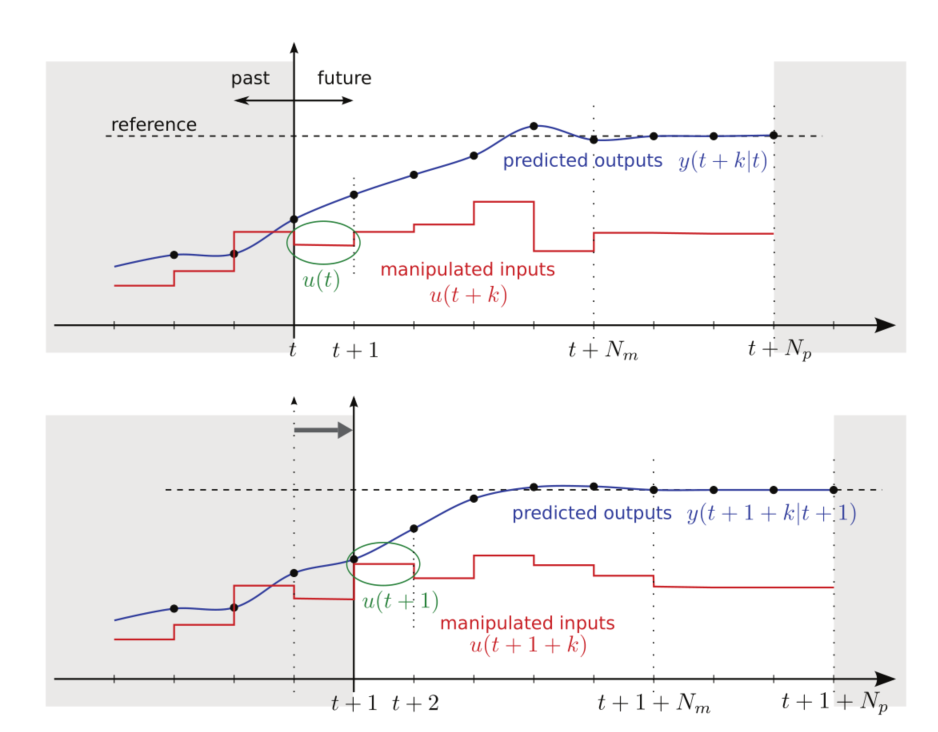
\includegraphics[width=.9\textwidth]{EMPC_PNG_Pics/RHC.png}
        \caption{Graphycal display of receiding horison control (RHC) idea \cite{borrelli2017predictive}.}
        \label{BASICCSR:fig:RHC}
    \end{figure}

The Formulation of the optimal control problem with moving horizon \cite{goodwin2006constrained} in the system \ref{BASICMPC:equ:basic_LTI} with input and output constraints as mentioned in \ref{BASICMPC:equ:basic_LTI_constrained} with the cost function to minimize:
		
		\begin{equation}
        \begin{array}{rcl}
				J(\textbf{U},\textbf{x}(q))&=&\min_{\textbf{U}_{q\rightarrow q+N|q}}J_q(\textbf{x}(q),\textbf{U}_{q\rightarrow q+N|q})\\
                &=&\textbf{x}'_{q+N_y|q}\textbf{P}\textbf{x}_{q+N_y|q}+\sum^{N_y-1}_{k=0}\textbf{x}'_{q+k|q}\textbf{Q}\textbf{x}_{q+k|q}+\textbf{u}'_{q+k}\textbf{R}\textbf{u}_{q+k},\\
				&\textnormal{subj. to}&\textbf{x}_N\in\mathcal{X}_f,\textbf{x}_k\in\mathcal{X}^x,\textbf{u}_k\in\mathcal{U}^u\\
				&&\textbf{x}_{q|q}=\textbf{x}(q),\\
				&&\textbf{x}_{q+k+1|q}=\textbf{A}\textbf{x}_{q+k|q}+\textbf{B}\textbf{u}_{q+k},\\
				%&&\textbf{y}_{q+k|q}=\textbf{C}\textbf{x}_{q+k|q}, k\geq0,\\
				&&\textbf{u}_{q+k}=-K\textbf{x}_{q+k|q}, N_u\leq k\leq N_y,\\
        \end{array}
        \label{BASICMPC:equ:receiding_horison_problem}
    \end{equation}
		
		where $\textbf{Q}=\textbf{Q}'\geq0$, $\textbf{R}=\textbf{R}'\geq0$, $\textbf{P}\geq0$, $(\textbf{C},\textbf{A})$ is observable, and $N_u\leq N_y$, $N_c\leq N_y-1$. One trivial possibility to choose $K=0$ and $\textbf{P}$ to satisfy the Lyapunov equation:
		
		\begin{equation}
        \begin{array}{rcl}
				\textbf{P}&=&\textbf{A}'\textbf{PA}+\textbf{Q}\\
        \end{array}
        \label{BASICMPC:equ:receiding_horison_Lyapunov}
    \end{equation}
		
		This means that after $N_u$ samples the control stops and the system is evolving to an open loop form. It is obvious that the choice only makes sense if the open loop system is stable. The second option would as described in \ref{BASICMPC:equ:control_coefficient_infinite}, and \ref{BASICMPC:equ:Riccati_infinite}, but this involves to use an unconstrained control for $N_u$ LQR samples. As a result, the MPC law calculates the optimal command sequence:
		
		\begin{equation}
        \begin{array}{rcl}
				\textbf{U}^*(q)&=&\left\{\textbf{u}^*_q,\dots,\textbf{u}^*_{q+N_u-1}\right\},\\
        \end{array}
        \label{BASICMPC:equ:receiding_optimal_sequence}
    \end{equation}
		
		and only the first control input is applied:
		
		\begin{equation}
        \begin{array}{rcl}
				\textbf{u}(q)=\textbf{u}^*_q.\\
        \end{array}
        \label{BASICMPC:equ:receiding_optimal_first}
    \end{equation}
		
		The optimal control inputs estimated for future samples are not taken into account and the algorithm is
repeated on the basis of new measurements or a new estimation of the states.	
    
    \subsubsection{Stability of MPC}\label{BASICCSR:sec:MPCStability}
    
    	The problem of closed system stability with the predictive control has been extensively studied e.g. in \cite{mayne2000constrained}, \cite{grieder2005stabilizing}. In the first generation of model based controllers, stability was achieved more experimentally by choosing parameters based on previous studies and experiences. In 1988 the Lyapunov stability method for discrete systems were introduced \cite{keerthi1988optimal}, and in 1990 for continuous systems \cite{mayne1990receding} also for continuous systems. \\
    While asymptotic convergence $\lim_{k\rightarrow\infty}\textbf{x}_k=0$ is a desirable property, it is generally not sufficient in practice. We would also like a system to stay in a small neighborhood of the origin when it is disturbed by a little. Formally this is expressed as Lyapunov stability.\\
    For the autonomous system:
    
    \begin{equation}
    \begin{array}{rcl}
            \textbf{x}_{k+1}&=&g(\textbf{x}_k)\\
            &\textnormal{subj. to}&g(0)=0,
        \end{array}
        \label{BASICMPC:equ:autonom_system}
    \end{equation}
    
    the defnition of Lyapunov stability is for the equilibrium point $\textbf{x}=0$ of system \ref{BASICMPC:equ:autonom_system} is:
    \begin{itemize}
    \item stable if, for each $\epsilon>0$, there is a $\delta>0$ such that:
        \begin{equation}
        \begin{array}{c}
                \norm{\textbf{x}_0}<\delta\textnormal{ s.t.: }\norm{\textbf{x}_k}<\epsilon,\textnormal{ }\forall k\geq0.
            \end{array}
            \label{BASICMPC:equ:lyapunov_1}
        \end{equation}
        
    \item unstable if not stable
    
    \item asymptotically stable if in the set $\boldsymbol{\Omega}\subseteq\mathbb{R}^n$ if its stable and:
       \begin{equation}
        \begin{array}{c}
                \lim_{k\rightarrow\infty}\textbf{x}_k=0,\textnormal{ }\forall\textbf{x}_0\in\boldsymbol{\Omega}.
            \end{array}
            \label{BASICMPC:equ:lyapunov_2}
        \end{equation}
    
    \item globally asymptotically stable if it is asymptotically stable and $\boldsymbol{\Omega}=\mathbb{R}^n$
    
    \item exponentially stable if it is stable and there exist constants $\alpha>0$ and $\gamma\in(0,1)$ such that:
    \begin{equation}
        \begin{array}{c}
                \norm{\textbf{x}_0}<\delta\textnormal{ s.t.: }\norm{\textbf{x}_k}\leq\alpha\norm{\textbf{x}_0}\gamma^k,\textnormal{ }\forall k\geq0.
            \end{array}
            \label{BASICMPC:equ:lyapunov_3}
        \end{equation}
    
    
    \end{itemize}
    
    Usually to show Lyapunov stability of the origin for a particular system one constructs a so called Lyapunov function, i.e., a function satisfying the conditions of the following theorem:\\
    Consider the equilibrium point $\textbf{x}=0$ of system \ref{BASICMPC:equ:autonom_system}. Let $\boldsymbol{\Omega}\subset\mathbb{R}^n$ be a closed and bounded set containing the origin. Assume there exists a function $V:\mathbb{R}^n\rightarrow\mathbb{R}$ continuous at the origin, finite for every $\textbf{x}\in\boldsymbol{\Omega}$ and such that:
    
    \begin{equation}
        \begin{array}{l}
                \bullet\textnormal{ } V(0)=0\\
                \bullet\textnormal{ } V(\textbf{x})>0,\textnormal{ }\forall\textbf{x}\in\boldsymbol{\Omega}\textbackslash\{0\}\\
                \bullet\textnormal{ } V(\textbf{x}_{k+1})-V(\textbf{x}_{k})\leq-\alpha(\textbf{x}_k),\textnormal{ }\forall\textbf{x}\in\boldsymbol{\Omega}\textbackslash\{0\},
            \end{array}
            \label{BASICMPC:equ:lyapunov_4_1}
        \end{equation}
        
     where $\alpha:\mathbb{R}^n\rightarrow\mathbb{R}$ is a continuous positive definite function, then $\textbf{x}=0$ is asymptotically stable. As such a function satisfying \ref{BASICMPC:equ:lyapunov_4} is called a Lyapunov function.\\
     A similar theorem can be derived for global asymptotic stability i.e.: $\boldsymbol{\Omega}=\mathbb{R}^n$:
     Consider the equilibrium point $\textbf{x}=0$ of system \ref{BASICMPC:equ:autonom_system}. Let $\boldsymbol{\Omega}\subset\mathbb{R}^n$ be a closed and bounded set containing the origin. Assume there exists a function $V:\mathbb{R}^n\rightarrow\mathbb{R}$ continuous at the origin, finite for every $\textbf{x}\in\boldsymbol{\Omega}$ and such that:
     
     \begin{equation}
        \begin{array}{l}
                \bullet\textnormal{ }\norm{\textbf{x}}\rightarrow\infty,\textnormal{ s.t.: }V(\textbf{x})\rightarrow\infty\\
                \bullet\textnormal{ } V(0)=0\\
                \bullet\textnormal{ } V(\textbf{x})>0,\textnormal{ }\forall\textbf{x}\neq0\\
                \bullet\textnormal{ } V(\textbf{x}_{k+1})-V(\textbf{x}_{k})\leq-\alpha(\textbf{x}_k),\textnormal{ }\forall\textbf{x}\neq0,
            \end{array}
            \label{BASICMPC:equ:lyapunov_4_2}
        \end{equation}
     where $\alpha:\mathbb{R}^n\rightarrow\mathbb{R}$ is a continuous positive definite function, then $\textbf{x}=0$ is globally asymptotically stable.\\
     For linear systems a simple and effective Lyapunov function can be:
     
     \begin{equation}
        \begin{array}{rcl}
                V(\textbf{x})&=&\textbf{x}'\textbf{P}\textbf{x},\textbf{P}\succ 0,\\
            \end{array}
            \label{BASICMPC:equ:lyapunov_5}
        \end{equation}
    
    In order to test the satisfaction of the last point of \ref{BASICMPC:equ:lyapunov_4_2}, we compute:
    
    \begin{equation}
        \begin{array}{rcl}
                V(\textbf{x}_{k+1})-V(\textbf{x}_{k})&=&\textbf{x}'_{k+1}\textbf{P}\textbf{x}_{k+1}-\textbf{x}'_{k}\textbf{P}\textbf{x}_{k}\\
                &=&\textbf{x}'_{k}(\textbf{A}'\textbf{P}\textbf{A})\textbf{x}_{k}-\textbf{x}'_{k}\textbf{P}\textbf{x}_{k}\\
                &=&\textbf{x}'_{k}(\textbf{A}'\textbf{P}\textbf{A}-\textbf{P})\textbf{x}_{k},
            \end{array}
            \label{BASICMPC:equ:lyapunov_6}
        \end{equation}
    
    therefore, if \ref{BASICMPC:equ:lyapunov_5} holds true then:
    
    \begin{equation}
        \begin{array}{rcl}
                 \textbf{A}'\textbf{P}\textbf{A}-\textbf{P}&=&-\textbf{Q},\textbf{Q}\succ 0,\\
            \end{array}
            \label{BASICMPC:equ:lyapunov_7}
        \end{equation}

	which is referred as discrete time Lyapunov equation.
	%with the restrictions:
%	
%	\begin{equation}
%        \begin{array}{rcl}
%            \textbf{Ex}(q)+\textbf{Lu}(q)\leq \textbf{M}\\
%        \end{array}
%        \label{BASICMPC:equ:restrict_LTI}
%    \end{equation}
%		
%		where $q\geq0$ defines the discrete time instance and $\textbf{x}\in \mathbb{R}^n$, $\textbf{u}\in \mathbb{R}^m$, $\textbf{y}\in %\mathbb{R}^p$ are the states, inputs and outputs of the system respectively. \\
%	 We define the following cost function to optimize:
%		
%		\begin{equation}
%        \begin{array}{rcl}
%				%&&\norm{asd}
%         J(\textbf{U}_n,x(0))&=&\norm{{\textbf{Px}_N}}_\varsigma+\sum^{N-1}_{k=0}\norm{\textbf{Qx}_k}_\varsigma+\norm{\textbf{Ru}_k}_\varsigma\\
%        \end{array}
%        \label{BASICMPC:equ:cost_function}
%    \end{equation}
%		
%		The optimization problem \ref{BASICMPC:equ:cost_function} applies with restrictions as follows:
%		
%		\begin{equation}
%        \begin{array}{rcl}
%				J^*(\textbf{x}(0))&=&min_{\textbf{U}_N}J(\textbf{U}_n,\textbf{x}(0))\\
%					&a.i.&\textbf{Ex}_k+\textbf{Lu}_k\leq \textbf{M},k=0,\dots,N-1\\
%					&&\textbf{x}\in \mathcal{X}_f\\
%					&&\textbf{x}_{k+1}=\textbf{Ax}_k+\textbf{Bu}_k,k\geq0\\
%					&&\textbf{x}_0=\textbf{x}(0)\\
%        \end{array}
%        \label{BASICMPC:equ:optim_problem}
%    \end{equation}
%		%
%		where $N$ is the defined horizon, $x\in \mathcal{X}_f$ is the set if terminal states, $\textbf{U}_N=[u_0,u_1,\dots,u_{N-1}]\in\mathbb{R}^s,s=m*N$.\\
% In case of $\varsigma=2$ (Euclidean or square norm) $\textbf{Q}=\textbf{Q}'\geq0$, $\textbf{R}=\textbf{R}'\geq0$, $\textbf{P}\geq0$ and in case of $\varsigma=1$, $\textbf{Q}$,$\textbf{R}$, and $\textbf{P}$ shall be on maximum rank. As displayed, the MPC approach requires a numerical definition so that a precise calculation can be made, that is, which predicted input trajectory gives the lowest numerical value to the cost. The main requirement is that the cost depends on the future controls and that low values of cost imply good closed-loop performance good being defined for the process. Of course the choice of the cost affects the complexity of the implied optimization and this is also a consideration. For this reason 2-norm ($\varsigma=2$) measures are popular, as optimization is straightforward.\\
%		Based on the latter and on \ref{BASICMPC:equ:cost_function} and \ref{BASICMPC:equ:optim_problem} a classical linear quadratic regulator %(LQR) structure can be formulated with finite or infinite horison \cite{aastrom2013computer}, \cite{bela2005iranyitasi}, \cite{levine2018control}.
%		Let us consider the following:
%		
%		\begin{equation}
%        \begin{array}{c}
%         \varsigma=2, \left\{(\textbf{x},\textbf{u})\in\mathbb{R}^n+m:\textbf{Ex}+\textbf{Lu}\leq %\textbf{M}\right\}=\mathbb{R},\mathcal{X}_f=\mathbb{R}^n\\
%        \end{array}
%        \label{BASICMPC:equ:quadratic_case}
%    \end{equation}
%		
%		In this case the problem can be reduced to an unconstrained optimization with finite horizon with the control law:
%		
%		\begin{equation}
%        \begin{array}{rcl}
%         \textbf{u}^*(k)&=&K_k\textbf{x}(k), k=0,\dots,N-1\\
%        \end{array}
%        \label{BASICMPC:equ:control_law}
%    \end{equation}
%		
%		Where the control coefficient of the $k^th$ instance is $K_k$ can be given in the following form:
%		
%		\begin{equation}
%        \begin{array}{rcl}
%         K_k&=&-(\textbf{B}'\textbf{P}_{k+1}\textbf{B}+\textbf{R})^{-1}\textbf{B}'\textbf{P}_{k+1}A\\
%        \end{array}
%        \label{BASICMPC:equ:control_coefficient}
%    \end{equation}
%		
%		The positive semi-definite matrix $\textbf{P}_k$ is the solution of the Riccati equation:
%		
%		\begin{equation}
%        \begin{array}{rcl}
%        \textbf{P}_N&=&\textbf{P}\\
%				\textbf{P}_k&=&\textbf{A}'(\textbf{P}_{k+1}-\textbf{P}{k+1}\textbf{B}(\textbf{B}'\textbf{P}_{k+1}\textbf{B}+\textbf{R})^{-1}\textbf{B}'P_{k+1})\textbf{A}+\textbf{Q}\\
%        \end{array}
%        \label{BASICMPC:equ:Riccati}
%    \end{equation}
%		
%		whith the initial condition:
%		
%		\begin{equation}
%        \begin{array}{rcl}
%				J^*(\textbf{x}(0))&=&\textbf{x}(0)'\textbf{P}_0\textbf{x}(0)\\
%        \end{array}
%        \label{BASICMPC:equ:Riccati_initial}
%    \end{equation}
%		
%		If we choose $N\longrightarrow\infty$ and assume that $(\textbf{A},\textbf{B})$ are controllable and $(\textbf{A},\textbf{B})$ are observable, the optimization problem becomes an infinite horizon LQR whose solution can be written as:
%		
%		\begin{equation}
%        \begin{array}{rcl}
%         \textbf{u}^*(k)&=&K_k\textbf{x}(k), k=0,\dots,\infty\\
%        \end{array}
%        \label{BASICMPC:equ:control_law_infinite}
%    \end{equation}
%		
%		As such:
%		
%		\begin{equation}
%        \begin{array}{rcl}
%         K_k&=&-(\textbf{B}'\textbf{P}_\infty \textbf{B}+\textbf{R})^{-1}\textbf{B}'\textbf{P}_\infty \textbf{A}\\
%        \end{array}
%        \label{BASICMPC:equ:control_coefficient_infinite}
%    \end{equation}
%		
%		with $\textbf{P}$ as the unique solution of the Riccati equiation:
%		
%		\begin{equation}
%        \begin{array}{rcl}
%				\textbf{P}_\infty&=&\textbf{A}'(\textbf{P}_\infty-\textbf{P}\infty \textbf{B}(\textbf{B}'\textbf{P}_\infty \textbf{B}+\textbf{R})^{-1}\textbf{B}'\textbf{P}_\infty)\textbf{A}+\textbf{Q}\\
%        \end{array}
%        \label{BASICMPC:equ:Riccati_infinite}
%    \end{equation}
%		
%		These are the basis of model predictive control (MPC). For introduction let us consider the principle of moving horizon (Receding Horizon). Optimization over a finite horizon has the following disadvantages:
%		
%		\begin{itemize}
%			\item Unforeseen problems may occur after the fixed optimization horizon, which may cancel the sequence of order for the 		calculated finished horizon.
%		\item After reaching the time defined by the horizon, the law of command is no longer optimal.
%		\item Finite horizon optimization is usually used because of the limited computing power is available, and not for theoretical reasons
%		\end{itemize}
%		
%		To prevent this problem, the notion of optimization is introduced on a moving horizon. In each sample $k$ , an optimization problem is solved over a defined horizon $k,\dots,k+N$ to calculate the appropriate command sequence, and only the first command is applied. This results in a moving optimization horizon, which eliminates the issues listed before. The Formulation of the optimal control problem with moving horizon \cite{goodwin2006constrained} in the system \ref{BASICMPC:equ:basic_LTI} with input and output constraints follows:
%		
%		\begin{equation}
%        \begin{array}{c}
%				\textbf{y}_{min}\leq \textbf{y}(t)\leq \textbf{y}_{max},\textbf{u}_{min}\leq \textbf{u}(t)\leq \textbf{u}_{max},\\
%        \end{array}
%        \label{BASICMPC:equ:receiding_horison_constraints}
%    \end{equation}
%		
%		
%with the cost function to minimize:
%		
%		\begin{equation}
%        \begin{array}{rcl}
%				J(\textbf{U},\textbf{x}(q)&=&\textbf{x}'_{q+N_y|q}\textbf{P}\textbf{x}_{q+N_y|q}+\sum^{N_y-1}_{k=0}\textbf{x}'_{q+k|q}\textbf{Q}\textbf{x}_{q+k|q}+\textbf{u}'_{q+k}\textbf{R}\textbf{u}_{q+k},\\
%				&a.i.&\textbf{y}_{min}\leq \textbf{y}_{q+k|q}\leq \textbf{y}_{ma\textbf{x}},k=1,\dots,N_c-1,\\
%				&&\textbf{u}_{min}\leq \textbf{u}_{q+k}\leq \textbf{u}_{max},k=0,1,\dots,N_c-1,\\
%				&&\textbf{x}_{q|q}=\textbf{x}(q),\\
%				&&\textbf{x}_{q+k+1|q}=\textbf{A}\textbf{x}_{q+k|q}+\textbf{B}\textbf{u}_{q+k},\\
%				&&\textbf{y}_{q+k|q}=\textbf{C}\textbf{x}_{q+k|q}, k\geq0,\\
%				&&\textbf{u}_{q+k}=-K\textbf{x}_{q+k|q}, N_u\leq k\leq N_y,\\
%        \end{array}
%        \label{BASICMPC:equ:receiding_horison_problem}
%    \end{equation}
%		
%		where $\textbf{Q}=\textbf{Q}'\geq0$, $\textbf{R}=\textbf{R}'\geq0$, $\textbf{P}\geq0$, $(\textbf{C},\textbf{A})$ is observable, [missing text] and $N_u\leq N_y$, $N_c\leq N_y-1$. One trivial possibility to choose $K=0$ and $\textbf{P}$ to satisfy the Lyapunov equation:
%		
%		\begin{equation}
%        \begin{array}{rcl}
%				\textbf{P}&=&\textbf{A}'\textbf{PA}+\textbf{Q}\\
%        \end{array}
%        \label{BASICMPC:equ:receiding_horison_Lyapunov}
%    \end{equation}
%		
%		This means that after $N_u$ samples the control stops and the system is evolving to an open loop form. It is obvious that the choice only makes sense if the open loop system is stable. The second option would as described in \ref{BASICMPC:equ:control_coefficient_infinite}, and \ref{BASICMPC:equ:Riccati_infinite}, but this involves to use an unconstrained control for $N_u$ LQR samples. As a result, the MPC law calculates the optimal command sequence:
%		
%		\begin{equation}
%        \begin{array}{rcl}
%				\textbf{U}^*(q)&=&\left\{\textbf{u}^*_q,\dots,\textbf{u}^*_{q+N_u-1}\right\},\\
%        \end{array}
%        \label{BASICMPC:equ:receiding_optimal_sequence}
%    \end{equation}
%		
%		and only the first control input is applied:
%		
%		\begin{equation}
%        \begin{array}{rcl}
%				\textbf{u}(q)=\textbf{u}^*_q.\\
%        \end{array}
%        \label{BASICMPC:equ:receiding_optimal_first}
%    \end{equation}
%		
%		The optimal control inputs estimated for future samples are not taken into account and the algorithm is
%repeated on the basis of new measurements or a new estimation of the states.

%\paragraph{Batch approach}


%\subsubsection{Stability of MPC}\label{BASICCSR:sec:MPCStability}		
%
%	The problem of closed system stability with the predictive control has been extensively studied e.g. in \cite{mayne2000constrained}, \cite{grieder2005stabilizing}. In the first generation of model based controllers, stability was achieved more experimentally by choosing parameters based on previous studies and experiences. In 1988 the Lyapunov stability method for discrete systems were introduced \cite{keerthi1988optimal}, and in 1990 for continuous systems \cite{mayne1990receding} also for continuous systems. \\
%	Generally, let $\textbf{U}\subset\mathbb{R}^n$ be an open set where $0\in \textbf{U}$. A function $V:\textbf{U}\longrightarrow\mathbb{R}$ is called positive (or negative) definite if $V(0)=0$ and $V(\boldsymbol{x})>0$ (or $V(\boldsymbol{x})<0$), when $\boldsymbol{x}\neq0$, and $\boldsymbol{x}\in U$. Also said function called positive (or negative) semidefinite if $V(0)=0$ and $V(\boldsymbol{x})\geq 0$ (or $V(\boldsymbol{x})\leq 0$), when $\boldsymbol{x}\neq 0$, and $\boldsymbol{x}\in \textbf{U}$. Clearly $V$ is a negative (semi-)definite function if $-V$ is a positive (semi-)definite function. So, in many applications the domain of $V$ is $\textbf{U}=\mathbb{R}^n$.\\
%	Also it can be said (according to the Sylvester theorem \cite{horn2012matrix}) that the quadratic function:
%	
%	\begin{equation}
%        \begin{array}{rcl}
%				V(\boldsymbol{x})&=&\boldsymbol{x}^T\boldsymbol{A}\boldsymbol{x},\\
%        \end{array}
%        \label{BASICMPC:equ:LyapunovTheory_0}
%    \end{equation}
%	
%	is positive definite iff all the leading principal minors if the matrix $A$ are positive. As such consider the nonlinear system \ref{BASICMPC:equ:LyapunovTheory_1}:
%	
%	\begin{equation}
%        \begin{array}{rcl}
%				\boldsymbol{\dot{x}}&=&f(\boldsymbol{x}),\\
%        \end{array}
%        \label{BASICMPC:equ:LyapunovTheory_1}
%    \end{equation}
%	
%	where we assume that $f(0)=0$ is a (trivial) equilibrium point of the system. The component functions of $f$ are denoted by $f(\boldsymbol{x})=f_1(\boldsymbol{x},\dots,f_n(\boldsymbol{x}))^T$. Let $V:\mathbb{R}^n\longrightarrow\mathbb{R}$ be continuously partially differentiable, with respect to all variables. By computing the derivative of the composite function $V(\boldsymbol{x}(t)$, where $\boldsymbol{x}(t)=(x_1(q),\dots,x_n(q)))^T$ is solution of \ref{BASICMPC:equ:LyapunovTheory_1}:
%	
%	\begin{equation}
%        \begin{array}{rcl}
%				\frac{dV}{dt}(\boldsymbol{x}(t))&=&\frac{\partial V}{\partial x_1}(\boldsymbol{x}(t)f_1(\boldsymbol{x}(t)))+\dots+\frac{\partial V}{\partial x_n}(\boldsymbol{x}(t)f_n(\boldsymbol{x}(t))),\\
%        \end{array}
%        \label{BASICMPC:equ:LyapunovTheory_2}
%    \end{equation}
%		
%		where the derivative of $V$ with respect to \ref{BASICMPC:equ:LyapunovTheory_1} follows:
%		
%		\begin{equation}
%        \begin{array}{rcl}
%				\dot{V}(\boldsymbol{x})&=&\frac{\partial V}{\partial x_1}(\boldsymbol{x}f_1(\boldsymbol{x}))+\dots+\frac{\partial V}{\partial x_n}(\boldsymbol{x}f_n(\boldsymbol{x})).\\
%        \end{array}
%        \label{BASICMPC:equ:LyapunovTheory_3}
%    \end{equation}
%		
%		If this function is negative definite then for every solution $\boldsymbol{x}(t)$ the composite function $V(\boldsymbol{x}(t))$ is monotone decreasing. Moreover, if  $V(\boldsymbol{x}(t))\longrightarrow 0$ as $t\longrightarrow \infty$, then $\boldsymbol{x}(t)\longrightarrow 0$ holds. This is the background of the next Lyapunov theorem:\\
%		Suppose $f(0)=0$, $\textbf{U}\subset\mathbb{R}^n$, is an open set with $0\in \textbf{U}$. Let $V:\textbf{U}\longrightarrow\mathbb{R}$ continuously differentiable with respect to all variables.
%		\begin{enumerate}[a)] % a), b), c), ...
%		\item If $V$ is positive definite and $\dot{V}$ is negative semidefinite, then the equlibrium $0$ of \ref{BASICMPC:equ:LyapunovTheory_1} is stable.
%		\item If $V$ is positive definite and $\dot{V}$ is negative definite, then the equlibrium $0$ of \ref{BASICMPC:equ:LyapunovTheory_1} is asymptotically stable.
%		\item If in every neighborhood of $0$ there exsists $\boldsymbol{x}$ such that $V(\boldsymbol{x})>0$ and $\dot{V}$ is positive definite, then the equlibrium $0$ of \ref{BASICMPC:equ:LyapunovTheory_1} is unstable.
%\end{enumerate}
%
%This way $V$ is called Lyapunov function if its positive definite and its derivative $\dot{V}$ with respect to \ref{BASICMPC:equ:LyapunovTheory_1} is negative semidefinite.\\
%	In this fashion, by using cost function, as a candidate for Lyapunov function, several methods of analysis have been developed, guaranteeing stability.	As basis the unconstrained LQR \ref{BASICMPC:equ:cost_function} is serving to create the Lypunov function such as:
%	
%\begin{equation}
%        \begin{array}{rcl}
%				V(x)&=&x'Px, P\succ 0.\\
%        \end{array}
%        \label{BASICMPC:equ:stability_Lyapunov_1}
%    \end{equation}
%		
%	In order to test this lets make the following calculation:
%	
%	\begin{equation}
%        \begin{array}{rcl}
%				V(x_{k+1})-V(x_{k})&=&x'_{k+1}Px_{k+1}-x'_{k}Px_{k}=\\
%				&=&k'_kA'PAx_k-x'_kPx_k=\\
%				&=&x'_k(A'PA-P)x_k,\\
%        \end{array}
%        \label{BASICMPC:equ:stability_Lyapunov_2}
%    \end{equation}
%		
%		where, in order to satisfy the Lyapunov theorem:
%		
%		\begin{equation}
%        \begin{array}{rcl}
%				A'PA-P&=&-Q, Q\succ 0.\\
%        \end{array}
%        \label{BASICMPC:equ:stability_Lyapunov_3}
%    \end{equation}
%		
%	This is referred to as discrete-time Lyapunov equation, where  according to \cite{borrelli2017predictive} iff $\textbf{P}$ satisfying \ref{BASICMPC:equ:stability_Lyapunov_3}, then the system is asymptotically stable. From an optimisation point of view problem \ref{BASICMPC:equ:optim_problem} in compact form:
%	
%\begin{equation}
%        \begin{array}{rcl}
%				%min_\textbf{U}J(\textbf{U},\textbf{x})&=&F(\textbf{x}_N)+\sum^{N-1}_{k=0}L(\textbf{x}_k,\textbf{u}_k)\\
%				\min_{\textbf{U}}J(\textbf{U},\textbf{x})&=&F(\textbf{x}_N)+\sum^{N-1}_{k=0}L(\textbf{x}_k,\textbf{u}_k)\\
%					&a.i.&\textbf{x}_{k+1}=f(\textbf{x}_k,\textbf{u}_k) \\
%					&&x\in \mathcal{X}_f, u\in \textbf{U}\\
%					&&\textbf{x}_0=\textbf{x}(q)\\
%        \end{array}
%        \label{BASICMPC:equ:optim_stability}
%    \end{equation}
%
%Assuming that the function cost $J(\textbf{U},\textbf{x})$ is a Lyapunov candidate, the MPC would be asymptotically make the system stable, if the following conditions are met:
%\begin{enumerate}
%	\item There is a terminal set $\Omega\subset \mathcal{X}_f$ so that $\Omega$ is also marginalized $0\in\Omega$ (constraints of states are satisfied in $\Omega$).
%	\item There is a terminal controller $K(\textbf{x}_k)\in U, \forall x\in\Omega,k=N,\dots,\infty$ (constraints of inputs are satisfied in $\Omega$)
%	\item The set $\Omega$ is invariant for the function $f(\textbf{x}_k,K(\textbf{x}_k)$ which needs to be optimized, so for every $\textbf{x}_0\in\Omega$, all subsequent $\textbf{x}_{k+1}=f(\textbf{x}_k,K(\textbf{x}_k)$ would remain in $\Omega$.
%	\item $F(f(\textbf{x}_k,K(\textbf{x}_k)))-F(\textbf{x})+L(\textbf{x}_k,K(\textbf{x}_k))\leq 0$, then $F()$ is the Lyapunov function in $\Omega$.
%\end{enumerate}
%
%Based on these conditions above, there are several methods of stabilizing the systems with MPC regulators, some of these are presented below \cite{herceg2009real}.
%
%\begin{itemize}
%	\item \textbf{MPC with final state constraint}: Stability is ensured by $\textbf{x}_N=0$. This imposes that $\Omega=\{0\}$, as such $K(\textbf{x}_k)=0$ maintains the state of origin. The advantage of the method is that we have a simple constraint, but imposing an equality constraint can to lead to difficulties in obtaining the solution.
%	\item \textbf{MPC with terminal cost}: This method imposes a zero terminal cost, without imposing restrictions
%for the final states. This method guarantees stability for large prediction horizons
%of unrestricted systems.
%	\item \textbf{MPC with permissible set restrictions of final states}: For this, it is required to $\textbf{x}_N\in\Omega$. This equality constraint ensures that the controller $K(\textbf{x}_k)$ remains in $\Omega$. This method is also called dual predictive controller, because two regulators are used, one with a moving horizon and one with stabilization of $K(\textbf{x}_k)$.
%	\item \textbf{MPC with permissible set restrictions on final states and terminal cost}: Combined method, and widely used because it encompasses the advantages of previous methods.
%\end{itemize}
%
%There are also stabilization methods such as infinite horizon MPCs or suboptimal MPC regulators, but we do not detail these methods because they are not mentioned in the thesis.
%
%\subsection{Explicit model predictive control (EMPC)}\label{BASICCSR:sec:EMPC}
%
%The problem \ref{BASICMPC:equ:receiding_horison_problem} can be transformed into a multi-parametric quadratic programming (mp-QP) problem. Such an approach involves solving the problem "offline", i.e. explicitly for the defined state-space with considering given constraints. By solving the optimization, critical regions are obtained, where each region corresponds to an optimal command that can be expressed as a function tuned by system states. Therefore the real-time regulation of the system is reduced to the identification of the critical regions corresponding to the measured state and the application of the optimal control input stored in a table. This method has revolutionized the use of the MPC method for systems with high dynamics, in particular for reduced order systems. The disadvantage of the method is that the number of critical regions increases exponentially with an increasing system order. The following shows the transformation of MPC into mp-QP.
%Let us assume an optimization problem described by \ref{BASICMPC:equ:receiding_horison_problem}. The evolution of the subsequent states is calculated according to the relation:
%
%\begin{equation}
%        \begin{array}{rcl}
%				\textbf{x}_{q+k|t}&=&\textbf{A}^k\textbf{x}(q)+\sum^{k-1}_{j=0}\textbf{A}^j\textbf{Bu}_{q+k-1-j}
%        \end{array}
%        \label{BASICMPC:equ:EMPC_evolution}
%    \end{equation}
%
%Based on \ref{BASICMPC:equ:receiding_horison_problem}, and \ref{BASICMPC:equ:EMPC_evolution} the optimization problem becomes:
%
%\begin{equation}
%        \begin{array}{rcl}
%				\textbf{V}(\textbf{x}(q))&=&\frac{1}{2}\textbf{x}'(q)\textbf{Yx}(q)+min\left\{\frac{1}{2}\textbf{U}'\textbf{HU}+\textbf{x}'(q)\textbf{FU}\right\},\\
%				%&with\,restrictions:&\textbf{GU}\leq \textbf{W}+\textbf{Ex}(t)\\
%        \end{array}
%        \label{BASICMPC:equ:EMPC_transformed}
%    \end{equation}
%		
%		with restrictions:
%		
%		\begin{equation}
%        \begin{array}{rcl}
%				\textbf{GU}&\leq& \textbf{W}+\textbf{Ex}(q),\\
%        \end{array}
%        \label{BASICMPC:equ:EMPC_transformed_2}
%    \end{equation}
%		
%		where $\textbf{U}=\{u'_t,\dots,u'_{q+N_u-1}\}\in\mathbb{R}^s,\,s=m\cdot N_u$, and $\textbf{H}$ is the optimization vector where $\textbf{H}=\textbf{H}'>0$, and $\textbf{H},\textbf{F},\textbf{Y},\textbf{G},\textbf{W},\textbf{E}$ can be directly obtained from $\textbf{A},\textbf{B},\textbf{Q},\textbf{R},\textbf{P}$, according to \cite{borrelli2017predictive}. Let the transformation vector be:
%		
%		\begin{equation}
%        \begin{array}{rcl}
%				\textbf{z}&=&\textbf{U}+\textbf{H}^{-1}\textbf{F}'\textbf{x}(q)
%        \end{array}
%        \label{BASICMPC:equ:EMPC_trans_var}
%    \end{equation}
%		
%		the cost function \ref{BASICMPC:equ:EMPC_transformed} becomes:
%		
%		\begin{equation}
%        \begin{array}{rcl}
%				\textbf{V}(\textbf{x})&=&\textbf{V}_z(\textbf{x})+\frac{1}{2}\textbf{x}'\left(\textbf{Y}-\textbf{FH}^{-1}\textbf{F}'\right)\textbf{x},
%        \end{array}
%        \label{BASICMPC:equ:EMPC_trans_var}
%    \end{equation}
%		
%		where $\textbf{V}_z(\textbf{x})$ is defined as:
%		
%		\begin{equation}
%        \begin{array}{rcl}
%				\textbf{V}_z(\textbf{x})&=&min\frac{1}{2}\textbf{z}'\textbf{Hz}\\
%				&s.t.&\textbf{Gz}\leq \textbf{W}+\textbf{Sx}(q)\\
%				&&\textbf{S}=\textbf{E}+\textbf{GH}^{-1}\textbf{F}'.\\
%        \end{array}
%        \label{BASICMPC:equ:EMPC_transformed}
%    \end{equation}
%		
%		From \ref{BASICMPC:equ:EMPC_transformed} the standard mp-QP problem can be defined according to \cite{borrelli2017predictive}, and through this transformation the MPC problem can be explicitly obtained.
		

\subsection{Storage of critical regions}\label{BASICCSR:sec:EMPCStorage}

The issue of iterative model based controllers is that they require a lot of computational resource. The CPU load and required ROM consumption could increase exponentially the longer the more steps the control horizon is calculated. For this reason explicit model bssed predictive controllers (EMPC) were developed, where only the storage the critical regions and the signal coefficients for each critical region, so the matrices $H$, $K$, $F$, $G$ are required. The on-line part of control consists of searching the critical region for the current states and calculating the necessary inputs for them.
One method of storing entire critical regions in order to calculate them, and that is in the order in which the MP-LP or MP-QP problem is resolved. It has the disadvantage, that the search time can be high, as such starting from the top of the list, a linear search is not effective. The efficient method is to store critical regions already in a binary tree \cite{jones2006logarithmic}, \cite{tondel2003evaluation}, \cite{tondel2003constrained}, \cite{kutasi2008vector}. The method of generating the binary tree is shown in (Fig.\ref{BASICMPC:fig:searchtree}.).\\
 The basic idea is to sort the critical regions depending on their adjacent sides. For example, in (Fig.\ref{BASICMPC:fig:searchtree}.a.) side $j_1$ divides the state space into two, at the right of it are the regions $X_{2,3,4,5}$ and to the left are the regions $X_{1,2,6}$. They make up the nodes adjacent to the base node $I_1$ of the binary tree. Next the another side from the space is chosen defined by each node $I_2$ respectively $I_3$, and the algorithm is continued until all the regions in the current node correspond to the same control signal, denoted by $F$ on the shaft in fig. (Fig.\ref{BASICMPC:fig:searchtree}.b.) Thus with this search pattern logarithmic search time can be achieved.

 \begin{figure}[!ht]
        \centering
        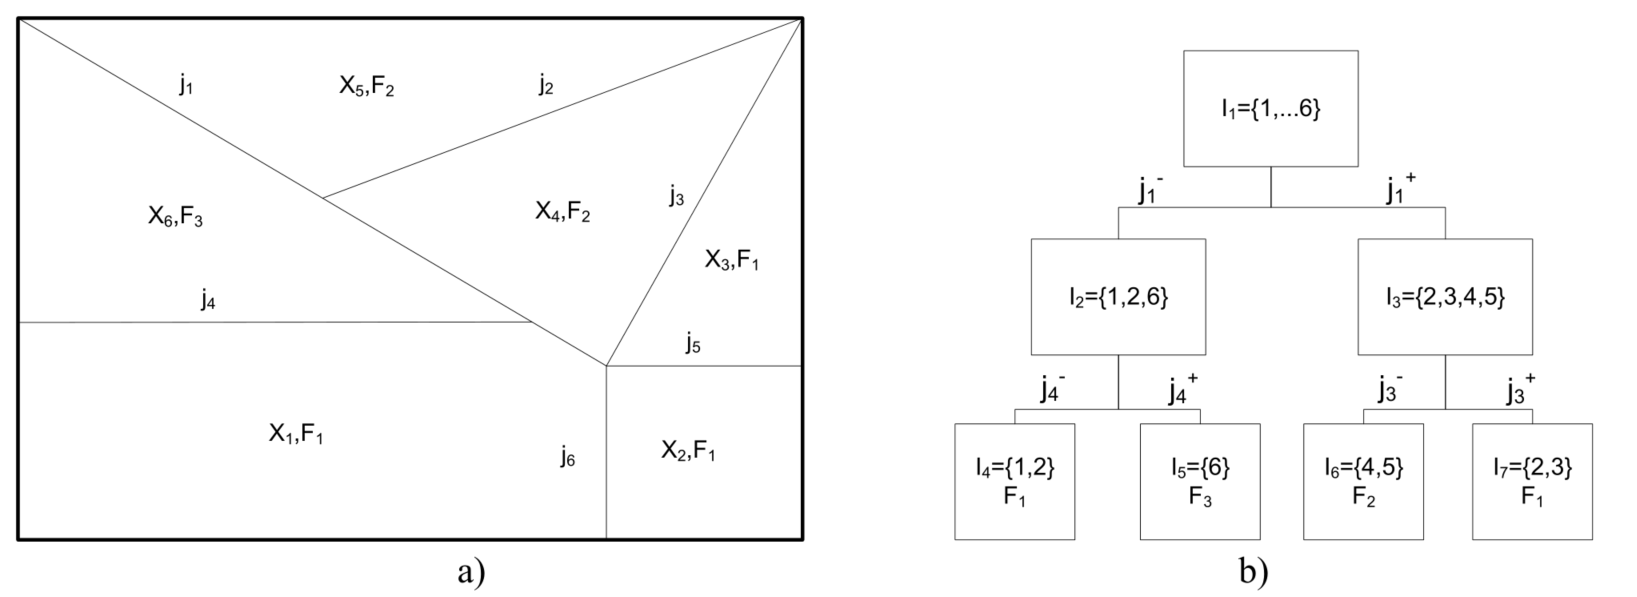
\includegraphics[width=\textwidth]{EMPC_PNG_Pics/BasicSearchTree.png}
        \caption{Basic search three of an EMPC where, a) are the critical regions for a space of 2D parameters,
b) the related binary tree.}
        \label{BASICMPC:fig:searchtree}
    \end{figure}

The implementation of MPC in explicit form is very efficient up to a certain number of critical regions, because they do not require calculations but only search in a table. For more complex problems or fast systems the method requires longer search time.

\section{Notations}

%\begin{table}[]
  %\centering
  %\caption{My caption}
  %\label{my-label}
%\begin{adjustbox}{width=\textwidth}
\begin{scriptsize}
\begin{tabularx}{\textwidth}{r|X}

  % after \\: \hline or \cline{col1-col2} \cline{col3-col4} ...
  %Chapter 4.1. notations&\\
	$V_P$															& Voltage peak\\
	$V12, V23, V31$										& Voltage vectors in the three phase phasor\\
  $VUFactor,VU,VUR$                	& Non standardized voltage unbalance factor based on manufacturer standards\\
	$V_{ab},V_{bc},V_{ca}$  					& Line-to-line voltages\\
	$V_{avg_{line}}$  								& Average of line voltages\\
	$LVUR$														& Voltage unbalance notation based on NEMA standard\\
	$PVUR_{IEEE-141},PVUR_{IEEE-936}$	& Voltage unbalance notation based on IEEE-141, and IEEE-936 standard\\
	$V_{a},V_{b},V_{c}$  							& Phase-to-neutral voltages\\
	$V_{avg_{phase}}$  								& Average of phase voltages\\
	$V_{0},V_{p},V_{n}$  							& Zero, negative and positive sequence voltages based on symmetrical components theorem\\
  $\upsilon$  											& Fortesque operator\\
	$VUF$  														& Voltage Unbalance Factor\\
	$CVUF$  													& Complex Voltage Unbalance Factor\\
	$k_v$  														& Magnitude of CVUF\\
	$\theta_v$  											& Angle of CVUF\\
	$i_i$															& Constant input inductor current\\
	$i_o$															& Alternating output current\\
	$V_i$															& Constant input voltage\\
	$V_o$															& Alternating output voltage\\
	$\frac{dV}{dt}$										& Derivative of voltage over time\\
	$L_+,L_-$													& Current filter inductors\\
	$S_{1+},S_{2+}$										& Higher switches\\
	$S_{1+},S_{2+}$										& Lower switches\\
	$D_{1+},D_{2+}$										& Higher diodes\\
	$D_{1+},D_{2+}$										& Lower diodes\\
	$v_\Delta$												& ???\\
	$v_c$															& ???\\
	$V_{an},V_{bn}$  									& Designated point's potential to ground on the CSI (Fig.\ref{BASICCSR:fig:SingleCSI}.)\\
	$\omega$													& Angular velocity of output sinusodial voltage or current\\
	$V_{D1},V_{D2}$ 									& Two end's voltage on the DC-DC converter\\
	$v_1,v_2$                         & Transformer voltages\\
	$C_{snub}$ 												& Capacitance to reduce switching loss and to damp out over-voltage\\
	$n$ 															& Transformer turn ratio.\\
	$L_a$															& Leakage inductance\\
	$v_D$															& Output voltage before the choke inductor $L_D$\\
	$V_d$															& Output voltage\\
	$I_D$															& Output current\\
	$L_D$															& Inductor for filtering the output current of the CSR (Choke)\\
	$C_D$															& Capacitance for filtering the output voltage of the VSR\\
	$L_S$															& Input filter inductance of the three phase alternating current in VSR\\
	$C_S$															& Input filter capacitance of the three phase alternating current in CSR\\
	$v_{c_p}$													& AC-side capacitor voltage, where $p\in\{1,2,3\}$\\
	$\widehat{u}$											& Peak value of AC-side capacitor voltage\\
	$v_{i,j}$													& Three phase phase-to-neutral voltage $i,j\in\{R,S,T\}$\\
	$v_{N,RS}$												& Three phase line-to-line voltage of $R$ and $S$\\
	$\varphi_N$												& Angle of phase voltage\\
	$\vec{i}$													& Rectifier input current\\
	$\vec{i}_ref$											& Reference rectifier input current\\
	$x$																& State\\
	$f(x)$														& Function of the state\\
	$\rho$																& Infinite sequence iterator\\
	$\Delta$													& Step lenght control parameter\\
	$\mathcal{P},\mathcal{D},\mathcal{S},\mathcal{Q},\mathcal{U},\mathcal{I},\mathcal{E}$ & Set of processes, directions, succesful iterations, timestep index, internal successes, and external succeses respectively\\
	$p$																& Process number\\
	$i$																& Active process indicator\\
	$d_i$															& Direction of active process\\
	$x_i^{best}$											& Best reached state, where $x_i^{best}$ is a minima\\
	$\Delta_i^{best}$											& Best reached step size\\
	$q$																& Discrete time step\\
	$\omega_i(q)$ 										& Generating process index for the update time at step $q$ on process $i$\\
	$\tau_i(q)$												& Time index for initialization of the function evaluation, that produced the update at time $q$ on process $i$\\
	$\nu_i(q)$ 												& Time index for the completion of the function evaluation that produced the update at time step $q$ on process $i$\\
	$\textbf{A}$																& State matrix\\
	$\textbf{B}$																& Input matrix\\
	$\textbf{C}$																& Output matrix\\
	$\textbf{x}$											& State vector\\
	$\textbf{z}$											& Input vector\\
	%$t$																& Time instance\\
	$\textbf{P}, \textbf{Q},\textbf{R}$ & Terminal, state, and input weight matrices respectively\\
	$\textbf{E}$																&???\\
	$\textbf{L}$																&???\\
	$\textbf{M}$																&???\\
	$\textbf{H}$																&???\\
	$\textbf{F}$																&???\\
	$\textbf{Y}$																&???\\
	$\textbf{G}$																&???\\
	$\textbf{W}$																&???\\
	$\textbf{E}$																&???\\
	$N$											& Defined horizon of MPC\\
	$N_c,N_u,N_y$											& Defined control, input, and output horizon of MPC respectively\\
	$k$																& Time step on the horison $N$ \\
	$\mathcal{X}_f$															& Set of terminal states \\
	$\textbf{U}_N$										& Vector of inputs sequence following the horizon\\
	$\varsigma$											& Norm index\\
	$s$																& ???\\
	$m$																& ???\\
	$K$															& Control coefficient \\
	$u^*(k)$													& $k^th$ instance of the optimizer input\\
	$\textbf{U}^*(k)$									& Optimal command sequence\\
	$\textbf{P}$																& Solution of the Riccati equation\\
	$\textbf{u}_{min,max},\textbf{y}_{min,max}$					& Input and output constraints\\
	$V(\textbf{x})$														& Lyapunov function of $\textbf{x}$\\
	$\Omega$ 													& Terminal set\\
	$\textbf{z}$																& transformation vector\\
	$X_j$															& $j^{th}$ resulting region after partitioning of the statespace\\
	$I_i$															& $i^{th}$ resulting node after partitioning of the statespace\\
	
\end{tabularx}
\end{scriptsize}
%\end{adjustbox}
%\end{table}

%\section{Summary}
%
%$\longmapsto$Summary of basic notions general.

